% !TeX root = ../../Book1.tex
% 纲要标题：## 第3章　凸性、多面体与有限维几何方法
% 纲要位置：几何学计划纲要.md，第 200 行。
% 正文状态：初稿；尚未正式审核。

% 纲要内容开始
% 
% > 本章目标与证明范围：以分离、有限支撑与对偶为主线，完整证明所选有限维分离定理、Carathéodory、Radon 和 Helly 定理。把群作用移至第1章，避免与凸几何并列拼接。
% 
% 纲要内容结束

\chapter{凸性、多面体与有限维几何方法}
\label{g1:ch:03}
\BookChapterNumber{g1:ch:03}

\begin{chapterabstract}
	凸性要求两点之间的整条线段留在集合内，却能把许多整体问题转成线性不等式。最近点投影产生支撑与分离超平面；仿射依赖限制凸组合所需的点数，并控制有限凸集族的相交；多面体则把这些方法收束为有限个顶点与有限个半空间之间的转换。面与法锥记录边界结构，极体把包含关系反转。最后，距离公式、环面作用的线性模型和格点的单项式映射展示这些方法如何进入后续几何。
\end{chapterabstract}

\begin{learninggoals}
	\begin{itemize}
		\item 区分内部与相对内部，证明闭凸集的最近点存在且唯一，并从投影不等式构造支撑及分离超平面。
		\item 说明弱分离、严格分离和有正间隔的分离各需要什么条件，识别闭性与紧性不能互换的情形。
		\item 利用仿射依赖完整证明 Carathéodory、Radon 和 Helly 定理，并用例子检验维数、凸性与有限族条件。
		\item 在有界情形证明半空间表示与顶点表示等价，计算面、法锥及极体，理解面对应为何反转包含关系。
		\item 用支撑函数计算距离，从整数权重计算矩映射的像，从格点关系写出射影方程。
	\end{itemize}
\end{learninggoals}

平面上的三角形
\[
	T=\{(x,y):x\ge0,\ y\ge0,\ x+y\le1\}
\]
既由三个不等式描述，又是三个点 \((0,0),(1,0),(0,1)\) 的凸包。后一种说法可以直接核验：若 \((x,y)\in T\)，则
\[
	(x,y)=(1-x-y)(0,0)+x(1,0)+y(0,1),
\]
三个系数非负且和为 \(1\)。不等式告诉我们哪些位置允许进入，顶点告诉我们如何生成所有允许的位置。更复杂的集合是否也有这两种描述？若一个点不在集合里，能否给出一条线性不等式作为证据？如果约束很多，又能否只看少量约束就判断它们不能同时满足？

\ProseParagraphBreak

本章逐步回答这些问题。先不要求集合由有限个条件给定，而从线段封闭这一性质出发。对非空闭凸集，集合外一点的最近点给出一个法向；这个法向产生的不等式把点与整个集合分开。接着利用有限维线性代数，把“点或条件太多”转化为依赖关系。最后回到有限个半空间的交，证明有界时可以恢复有限个顶点，并追踪边界各部分如何在对偶构造中交换角色。

\ProseParagraphBreak

所需的代数基础是仿射组合、秩、核与对偶空间。\cref{g1:prop:affine-combination}说明系数和为 \(1\) 的组合不依赖原点；本章再要求系数非负，从而保留线段内的位置。分析方面使用有限维欧氏空间中“闭且有界等价于紧”、紧集上连续实函数取得最值，以及有界序列有收敛子列；应用这些事实时会指出闭性与有界性从何而来。本章先在 \(\mathbb R^n\) 中证明所需结论，不要求泛函分析中的一般分离定理。凸集与分离的补充阅读可参看\cite[Sections 2.1, 2.5--2.6]{BoydVandenberghe2004}和\cite[Sections 3.1--3.2, 3.4, 7.1--7.2]{Gallier2011Geometric}；多面体的有限表示与面结构可参看\cite[Sections 1.1, 2.1--2.4]{Ziegler1995}。

% !TeX root = ../../Book1.tex
% 纲要标题：### 3.1 凸集、支撑与分离
% 纲要位置：几何学计划纲要.md，第 204 行。
% 正文状态：初稿；尚未正式审核。

% 纲要内容开始
% 
% * 凸包、相对内部和仿射包络
% * 最近点投影及支撑超平面
% * 凸集的弱分离、严格分离与强分离
% * 闭凸集的支撑函数表示
% 
% 纲要内容结束

\section{凸集、支撑与分离}
\label{g1:sec:0301}

在平面上围住一组点，可以用曲线描出边界，也可以逐个指定包含这些点的半平面。前一种描述关注边界在哪里，后一种描述关注各个方向上能走多远。对于凸集，两种描述能够互相恢复。证明这一点的关键是：若一个点在闭凸集之外，能否找到一个半空间，把整个集合留在一侧而把该点排除在外？本节从最近点出发构造这样的半空间。除特别说明外，环境为带标准内积的 \(\mathbb R^n\)，\(n\geq1\)，范数记为 \(\lVert\cdot\rVert\)。

\subsection{凸包、相对内部和仿射包络}
\label{g1:subsec:0301:01}

\cref{g1:prop:affine-combination}说明，系数和为 \(1\) 的仿射组合不依赖原点。若进一步要求系数非负，就不会沿着两点的连线越过端点。这一限制把仿射几何中的“张成”变成了凸几何中的“围住”。

\begin{definition}[凸集与凸包]\label{g1:def:convex-hull}
	设集合 \(C\subseteq\mathbb R^n\)。若对任意 \(x,y\in C\) 和 \(t\in[0,1]\)，都有 \((1-t)x+ty\in C\)，则称其为\term[tuji]{凸集}[convex set]。有限个点的仿射组合 \(\sum_{i=1}^m\lambda_i x_i\) 若满足 \(\lambda_i\geq0\)、\(\sum_i\lambda_i=1\)，称为\term[tuzuhe]{凸组合}[convex combination]。对任意 \(S\subseteq\mathbb R^n\)，其\term[tubao]{凸包}[convex hull] \(\operatorname{conv}S\) 是所有包含 \(S\) 的凸集之交。
	\symidx{\(\operatorname{conv}S\)：凸包}
\end{definition}

按定义，空集和单点集都是凸集；\(\operatorname{conv}\varnothing=\varnothing\)。任意一族凸集的交仍为凸集，因为交集中任意两点之间的线段属于这族集合的每一个成员。这里不要求集合闭：开球和闭球都凸，开球并不包含自己的边界。

\begin{proposition}[凸包的有限组合表示]\label{g1:prop:convex-finite-combinations}
	设 \(S\subseteq\mathbb R^n\) 非空，则
	\[
		\operatorname{conv}S=\left\{\,\sum_{i=1}^m\lambda_i x_i:m\geq1,\ x_i\in S,\ \lambda_i\geq0,\ \sum_{i=1}^m\lambda_i=1\,\right\}.
	\]
	此外，凸集的闭包仍为凸集，仿射映射把凸集映为凸集。
\end{proposition}
\begin{proof}
	先用点数归纳说明凸集包含其点的一切有限凸组合。一个点的情形成立。若 \(\lambda_m=1\)，组合等于 \(x_m\)；否则把前 \(m-1\) 项除以 \(1-\lambda_m>0\)，先得到归纳假设所允许的一个点，再与 \(x_m\) 作两点凸组合。因而上式右边包含于每个包含 \(S\) 的凸集中。

	反过来，右边包含 \(S\)，而两个有限凸组合再按权重 \(1-t,t\) 组合，只需把原来两组系数分别乘以 \(1-t,t\)，仍得到非负且总和为 \(1\) 的有限组系数。因此右边本身凸，由凸包的定义得到相等。

	若 \(x,y\in\overline C\)，取 \(x_j,y_j\in C\) 分别趋于 \(x,y\)。对固定 \(t\in[0,1]\)，点 \((1-t)x_j+ty_j\in C\) 趋于 \((1-t)x+ty\)，故极限在 \(\overline C\) 中。最后，\cref{g1:prop:affine-preservation}给出 \(f((1-t)x+ty)=(1-t)f(x)+tf(y)\)，因而 \(f(C)\) 凸。
\end{proof}

“有限”不是对集合 \(S\) 的限制，而是对每一个具体表示的限制；所需点数暂时可以依赖于所表示的点。另一个需要区分的概念是仿射包络。\secref{g1:sec:0101}末尾已说明，对非空 \(S\) 及 \(a\in S\)，
\[
	\operatorname{aff}S=a+\operatorname{span}\{x-a:x\in S\}.
\]
它允许系数为负的一切有限仿射组合，因而 \(\operatorname{conv}S\subseteq\operatorname{aff}S\)，且两者有相同的仿射包络。记 \(\dim C=\dim\operatorname{aff}C\)，此记号在这里用于非空凸集。

\begin{definition}[相对内部与相对边界]\label{g1:def:relative-interior}
	设非空集合 \(C\subseteq\mathbb R^n\) 的仿射包络为 \(F=a+L\)。它的\term[xiangduineibu]{相对内部}[relative interior]是它在 \(F\) 中的内部，记为
	\[
		\operatorname{ri}C=\{\,x\in C:\text{存在 }r>0\text{ 使 }\{x+v:v\in L,\ \lVert v\rVert<r\}\subseteq C\,\}.
	\]
	它的\term[xiangduibianjie]{相对边界}[relative boundary]为 \(\operatorname{rbd}C=\overline C\setminus\operatorname{ri}C\)。这里仿射子空间 \(F\) 在有限维 Euclid 空间中闭，故相对闭包与环境空间中的闭包相同。对空集约定 \(\operatorname{ri}\varnothing=\operatorname{rbd}\varnothing=\varnothing\)。
	\symidx{\(\operatorname{ri}C,\operatorname{rbd}C\)：相对内部与相对边界}
\end{definition}

\begin{example}[一条线段的两种内部]\label{g1:exm:relative-segment}
	令 \(C=\{(t,0):0\leq t\leq1\}\subseteq\mathbb R^2\)。平面中的任何小圆盘都不能放进 \(C\)，故 \(\operatorname{int}C=\varnothing\)，整个 \(C\) 都是环境空间中的边界。它的仿射包络却只是 \(x\) 轴，于是 \(\operatorname{ri}C=\{(t,0):0<t<1\}\)，相对边界只有两个端点。若 \(C=\{p\}\)，仿射包络是零维空间 \(\{p\}\)，相对内部等于 \(C\)，相对边界为空。所谓“内部”必须说明在哪个空间中计算。
\end{example}

\begin{proposition}[相对内部的存在与闭包]\label{g1:prop:relative-interior}
	设 \(C\subseteq\mathbb R^n\) 为非空凸集，\(F=\operatorname{aff}C\)。则 \(\operatorname{ri}C\ne\varnothing\)。若 \(a\in\operatorname{ri}C\)、\(b\in\overline C\) 和 \(0\leq t<1\)，则 \((1-t)a+tb\in\operatorname{ri}C\)。并且
	\[
		\overline{\operatorname{ri}C}=\overline C,\qquad
		\operatorname{ri}(\overline C)=\operatorname{ri}C.
	\]
\end{proposition}
\begin{proof}
	令 \(d=\dim F\)。当 \(d=0\) 时，\(C\) 为单点，全部结论成立。若 \(d\geq1\)，从 \(C\) 中逐次选择点，直至得到张成 \(F\) 的仿射无关组 \(p_0,\ldots,p_d\)：只要已有点的仿射包络不是 \(F\)，就还可从 \(C\) 选到包络之外的点，每次使维数增加一。由\cref{g1:prop:affine-coordinates}，相对于这组点的重心坐标 \(\lambda_i\) 是 \(F\) 上的连续仿射函数。重心 \(a=(p_0+\cdots+p_d)/(d+1)\) 的各坐标均为正，因此在 \(F\) 中的某个小球上各 \(\lambda_i\) 仍为正。这个小球包含于这些点的凸包，再包含于 \(C\)，故 \(a\in\operatorname{ri}C\)。

	现任取 \(a\in\operatorname{ri}C\)，选 \(r>0\) 使相对球 \(B_F(a,r)\subseteq C\)。固定 \(t<1\)，取 \(b_j\in C\) 趋于 \(b\)。由凸性，
	\[
		B_F((1-t)a+tb_j,(1-t)r)\subseteq C.
	\]
	当 \(j\) 充分大时，球心与 \((1-t)a+tb\) 的距离小于 \((1-t)r/2\)，故以后一个点为中心、半径为 \((1-t)r/2\) 的相对球仍包含于 \(C\)。这证明线段上除 \(b\) 外的各点都在相对内部。令 \(t\) 趋于 \(1\)，可知每个 \(b\in\overline C\) 都属于 \(\overline{\operatorname{ri}C}\)；反向包含来自 \(\operatorname{ri}C\subseteq C\)。

	由于 \(F\) 闭且 \(C\subseteq\overline C\subseteq F\)，\(\overline C\) 的仿射包络仍为 \(F\)，并有 \(\operatorname{ri}C\subseteq\operatorname{ri}(\overline C)\)。若 \(x\in\operatorname{ri}(\overline C)\)，固定一个 \(a\in\operatorname{ri}C\)。\(x=a\) 时无须再证；否则可取充分小的 \(\varepsilon>0\)，使 \(b=x+\varepsilon(x-a)\in\overline C\)。此时
	\[
		x=\frac{\varepsilon}{1+\varepsilon}a+\frac{1}{1+\varepsilon}b,
	\]
	右边是刚刚讨论过的线段内部点，故 \(x\in\operatorname{ri}C\)，得到最后一个等式。
\end{proof}

特别地，具有非空普通内部的凸集满足 \(\operatorname{int}(\overline C)=\operatorname{int}C\)。对这样的凸集，取闭包可以补入原来缺失的边界点，内部则保持不变。

\subsection{最近点投影及支撑超平面}
\label{g1:subsec:0301:02}

\cref{g1:prop:projection}给出子空间中的唯一最近点：把 \(x\) 分成沿子空间的分量和正交分量。对于一般凸集，最近点处不一定有一条可以向两边自由移动的直线，所以“与所有允许方向正交”需要改成“沿任何允许方向移动都不会缩短距离”。这会把等式条件变成一个内积不等式。

\begin{theorem}[闭凸集的最近点投影]\label{g1:thm:convex-projection}
	设 \(C\subseteq\mathbb R^n\) 为非空闭凸集。每个 \(x\in\mathbb R^n\) 都有唯一最近点 \(P_Cx\in C\)，满足
	\[
		\lVert x-P_Cx\rVert=d(x,C)\coloneqq\inf_{y\in C}\lVert x-y\rVert.
	\]
	而且，对 \(p\in C\)，有等价刻画
	\begin{equation}\label{g1:eq:convex-projection-variation}
		p=P_Cx\quad\Longleftrightarrow\quad
		\langle x-p,y-p\rangle\leq0\quad\text{对所有 }y\in C.
	\end{equation}
	因此对所有 \(y\in C\)，
	\begin{equation}\label{g1:eq:convex-projection-distance}
		\lVert x-y\rVert^2\geq\lVert x-P_Cx\rVert^2+\lVert y-P_Cx\rVert^2.
	\end{equation}
\end{theorem}
\begin{proof}
	先证明最小值能取到。取 \(c_0\in C\)，则 \(d(x,C)\leq\lVert x-c_0\rVert<\infty\)。按下确界定义可取 \(y_j\in C\)，使 \(\lVert x-y_j\rVert\to d(x,C)\)。这些距离有界，所以 \((y_j)\) 有界。有限维实分析中的有界序列子列定理保证它有收敛子列；因 \(C\) 闭，其极限 \(p\) 仍在 \(C\)，范数连续性给出 \(\lVert x-p\rVert=d(x,C)\)。这里没有要求整个 \(C\) 有界，只需要控制这一列候选点。

	若 \(p\) 是最近点，任取 \(y\in C\)。由凸性，\(p+t(y-p)\in C\) 对 \(0\leq t\leq1\) 成立，于是
	\[
		0\leq\lVert x-p-t(y-p)\rVert^2-\lVert x-p\rVert^2
		=-2t\langle x-p,y-p\rangle+t^2\lVert y-p\rVert^2.
	\]
	对 \(t>0\) 除以 \(t\)，再令 \(t\to0^+\)，得到所需内积不等式。反过来，若 \(p\in C\) 满足该不等式，则
	\[
		\lVert x-y\rVert^2
		=\lVert x-p\rVert^2+\lVert y-p\rVert^2-2\langle x-p,y-p\rangle
		\geq\lVert x-p\rVert^2+\lVert y-p\rVert^2.
	\]
	它首先说明 \(p\) 是最近点；若 \(y\) 也是最近点，左右最短距离相等，便迫使 \(\lVert y-p\rVert=0\)。这同时证明唯一性和最后一个不等式。
\end{proof}

映射 \(P_C\) 称为到 \(C\) 的\term[zuijindiantouying]{最近点投影}[nearest-point projection]。如果 \(C=W\) 是子空间，将 \(y=p+w\) 和 \(y=p-w\) 同时代入式\eqref{g1:eq:convex-projection-variation}，就得到 \(\langle x-p,w\rangle=0\)，恢复了第一章的正交投影。对于一般凸集，只能沿集合内部的方向移动，因此只能得到不等式。
\symidx{\(P_Cx\)：闭凸集的最近点投影}

\begin{example}[球上的投影及两项条件的作用]\label{g1:exm:ball-projection}
	对 \(C=\{y:\lVert y\rVert\leq r\}\)，其中 \(r>0\)，有
	\[
		P_Cx=\begin{cases}x,&\lVert x\rVert\leq r,\\[2pt]
		r x/\lVert x\rVert,&\lVert x\rVert>r.
		\end{cases}
	\]
	第二种情形中，令 \(p=rx/\lVert x\rVert\)，则 \(x-p\) 是 \(p\) 的正倍数，而对每个 \(y\in C\)，\(\langle p,y-p\rangle\leq r\lVert y\rVert-r^2\leq0\)，所以可用投影刻画验证该式。这个投影通常不是线性的。若把闭球改成开球，外点的距离下确界仍为 \(\lVert x\rVert-r\)，却没有最近点，说明闭性用于保证存在。若取闭集 \(C=\{-1,1\}\subseteq\mathbb R\)，则 \(0\) 有两个最近点，说明缺少凸性会破坏唯一性。
\end{example}

最近点还给出一个方向：从集合指向外点的向量 \(x-P_Cx\)。投影不等式说，整个集合都位于过 \(P_Cx\)、垂直于这个向量的超平面的一侧，如\cref{g1:fig:convex-separation}所示。

\begin{theorem}[点与闭凸集的分离]\label{g1:thm:point-closed-separation}
	设 \(C\subseteq\mathbb R^n\) 为非空闭凸集，\(x\notin C\)。令 \(p=P_Cx\)、\(u=(x-p)/\lVert x-p\rVert\)，则 \(\lVert u\rVert=1\)，且
	\begin{equation}\label{g1:eq:point-closed-separation}
		\langle u,y\rangle\leq\langle u,p\rangle
		<\langle u,x\rangle=\langle u,p\rangle+d(x,C)
		\quad(y\in C).
	\end{equation}
	特别地，存在 \(\alpha\in\mathbb R\) 和 \(\varepsilon>0\)，使 \(\langle u,y\rangle\leq\alpha-\varepsilon\) 对所有 \(y\in C\) 成立，而 \(\langle u,x\rangle\geq\alpha+\varepsilon\)。
\end{theorem}
\begin{proof}
	由 \(x\notin C\) 和最近点存在可知 \(x\ne p\)，故 \(d(x,C)=\lVert x-p\rVert>0\)。将式\eqref{g1:eq:convex-projection-variation}除以此正数，就得到 \(\langle u,y-p\rangle\leq0\)。同时 \(\langle u,x-p\rangle=\lVert x-p\rVert\)，得所示不等式。取 \(\alpha=(\langle u,p\rangle+\langle u,x\rangle)/2\)、\(\varepsilon=d(x,C)/2\) 即得最后一项。
\end{proof}

\begin{figure}[htbp]
	\centering
	% !TeX root = ../Book1.tex
\begin{tikzpicture}[scale=1.02,>=Stealth]
	\filldraw[fill=GeometryBlue!8,draw=GeometryBlue,thick] (0,0) ellipse (1.4 and 1.05);
	\node[GeometryBlue] at (-0.7,-0.35) {\(C\)};
	\draw[GeometryBlue,thick] (1.4,-1.5) -- (1.4,1.65);
	\draw[GeometryGray,dashed,thick] (2.7,-1.5) -- (2.7,1.65);
	\draw[->,thick] (1.4,0) -- (2.25,0) node[above,midway] {\(u\)};
	\draw[GeometryGray] (2.25,0) -- (4,0);
	\draw[->,GeometryBlue] (1.4,0) -- (-0.45,0.78);
	\fill (1.4,0) circle (1.6pt) node[below left] {\(p=P_Cx\)};
	\fill (4,0) circle (1.6pt) node[right] {\(x\)};
	\fill (-0.45,0.78) circle (1.6pt) node[above] {\(y\)};
	\node[align=center,font=\small] at (0.75,-1.85) {支撑超平面};
	\node[align=center,font=\small] at (3.25,-1.85) {分离超平面};
	\draw[GeometryGray,thin] (0.75,-1.65) -- (1.4,-1.45);
	\draw[GeometryGray,thin] (3.25,-1.65) -- (2.7,-1.45);
\end{tikzpicture}

	\caption[最近点、支撑超平面与分离超平面]{最近点、支撑超平面与分离超平面。实线过最近点 \(p\)，虚线位于 \(p\) 与外点 \(x\) 之间；\(C\) 中所有方向 \(y-p\) 与 \(x-p\) 的内积都非正。}
	\label{g1:fig:convex-separation}
\end{figure}

\begin{definition}[支撑超平面]\label{g1:def:supporting-hyperplane}
	设 \(C\subseteq\mathbb R^n\) 非空，\(p\in\overline C\)。若 \(u\ne0\)，且 \(\langle u,y\rangle\leq\langle u,p\rangle\) 对每个 \(y\in C\) 成立，则称
	\[
		H=\{y:\langle u,y\rangle=\langle u,p\rangle\}
	\]
	为 \(C\) 在 \(p\) 处的\term[zhichengchaopingmian]{支撑超平面}[supporting hyperplane]，向量 \(u\) 指向所选的外侧。
\end{definition}

定义允许整个 \(C\) 都在超平面上，因而也适用于低维集合。过最近点的超平面已经给出了某些支撑超平面，但一般边界点未必事先被表示成某个外点的投影。可以让外点趋近指定边界点，利用单位法向量的紧性留下一个极限方向。

\begin{theorem}[边界点的支撑超平面]\label{g1:thm:supporting-hyperplane}
	设 \(C\subseteq\mathbb R^n\) 为非空闭凸集。对每个 \(p\in\partial C\)，都存在 \(u\in\mathbb R^n\)、\(\lVert u\rVert=1\)，使
	\[
		\langle u,y-p\rangle\leq0\qquad(y\in C).
	\]
	若在 \(F=\operatorname{aff}C=a+L\) 中讨论，\(\dim F\geq1\)，则每个 \(p\in\operatorname{rbd}C\) 都有法向量 \(u\in L\setminus\{0\}\) 的相对支撑超平面；这个超平面不会包含整个 \(C\)。
\end{theorem}
\begin{proof}
	由 \(p\in\partial C\)，可选 \(x_j\notin C\) 且 \(x_j\to p\)。令 \(p_j=P_Cx_j\)。因为 \(p\in C\)，有
	\[
		\lVert p_j-p\rVert\leq\lVert p_j-x_j\rVert+\lVert x_j-p\rVert
		=d(x_j,C)+\lVert x_j-p\rVert\leq2\lVert x_j-p\rVert\to0.
	\]
	取单位向量 \(u_j=(x_j-p_j)/\lVert x_j-p_j\rVert\)。单位球面紧，故可取子列使 \(u_j\to u\)，其中 \(\lVert u\rVert=1\)。对任意固定 \(y\in C\)，投影刻画给出 \(\langle u_j,y-p_j\rangle\leq0\)，沿该子列取极限得 \(\langle u,y-p\rangle\leq0\)。同一个收敛子列对所有这些不等式都适用，因为选取它只用到了 \((u_j)\)，不依赖于 \(y\)。

	对相对边界，在 \(F\) 内选择趋于 \(p\) 的外点，并以 \(L\) 的标准正交坐标重复上述证明，所得单位法向量属于 \(L\)。若相应超平面包含整个 \(C\)，则 \(\langle u,y-p\rangle=0\) 对所有 \(y\in C\) 成立。由于 \(p\in C\) 且这些差向量张成 \(L\)，便有 \(u\perp L\)，与 \(0\ne u\in L\) 矛盾。
\end{proof}

普通边界与相对边界在这里给出不同信息。例如，线段的内点在平面中也有支撑直线，但这条直线只能包含整条线段；在其一维仿射包络内，它并不是边界点，也就不需要有支撑超平面。零维非空凸集没有相对边界，故相对版本在零维时没有待讨论的点。

\subsection{凸集的弱分离、严格分离与强分离}
\label{g1:subsec:0301:03}

分离两个集合时，“在两侧”可能只要求不越过同一个超平面，也可能要求两边各自留下间隙。先明确这些量词，才能判断闭性、开性或紧性分别解决什么问题。下列用语中的法向量总是非零向量，否则常数函数会给出毫无几何内容的等式。

\begin{definition}[分离的三种条件]\label{g1:def:convex-separation}
	设 \(A,B\subseteq\mathbb R^n\) 非空。
	\begin{enumerate}
		\item 若存在 \(u\ne0\)、\(\alpha\in\mathbb R\)，使 \(\langle u,a\rangle\leq\alpha\leq\langle u,b\rangle\) 对所有 \(a\in A,b\in B\) 成立，称 \(A,B\) 被该超平面\term[ruofenli]{弱分离}[weakly separated]。
		\item 若上述两个不等号对每个 \(a,b\) 都严格成立，称为\term[yangefenli]{严格分离}[strict separation]。
		\item 若存在 \(u\ne0\)、\(\alpha\in\mathbb R\)、\(\varepsilon>0\)，使 \(\langle u,a\rangle\leq\alpha-\varepsilon\) 且 \(\langle u,b\rangle\geq\alpha+\varepsilon\) 对所有 \(a,b\) 成立，称为\term[qiangfenli]{强分离}[strong separation]。
	\end{enumerate}
\end{definition}

强分离等价于存在 \(u\ne0\) 使 \(\sup_{a\in A}\langle u,a\rangle<\inf_{b\in B}\langle u,b\rangle\)：两个端值之间取中点和半间距即可。严格分离只要求逐点严格，两个端值仍可能相同。文献对“严格分离”和“强分离”的命名并不完全统一，本书按上面的量词区分；比较定理时应比较不等式本身。分离与支撑的基本观点可参阅 \cite[第2章，第2.5节]{BoydVandenberghe2004}。

\begin{theorem}[一个集合开时的弱分离]\label{g1:thm:convex-weak-separation}
	设 \(A,B\subseteq\mathbb R^n\) 为非空凸集，且至少一个为开集。则 \(A\cap B=\varnothing\) 当且仅当它们可以弱分离。若 \(A\) 开，分离不等式在 \(A\) 一侧必严格；若 \(B\) 开，在 \(B\) 一侧必严格。
\end{theorem}
\begin{proof}
	先设 \(A\cap B=\varnothing\)，考虑差集
	\[
		D=B-A=\{b-a:a\in A,\ b\in B\}.
	\]
	分别对两个分量取凸组合可知 \(D\) 凸。若 \(B\) 开，\(D=\bigcup_{a\in A}(B-a)\) 是开集；若 \(A\) 开，改用 \(D=\bigcup_{b\in B}(b-A)\) 得到同一结论。\(D\) 非空，且 \(0\notin D\)。由\cref{g1:prop:relative-interior}在满维开凸集上的结论，\(\operatorname{int}\overline D=D\)。因此 \(0\) 要么在闭凸集 \(\overline D\) 之外，要么在它的边界。

	若 \(0\notin\overline D\)，应用\cref{g1:thm:point-closed-separation}并把法向量反向，得到某个 \(u\ne0\)，使 \(\langle u,d\rangle>0\) 对所有 \(d\in D\) 成立。若 \(0\in\partial\overline D\)，则对 \(\overline D\) 在 \(0\) 处应用\cref{g1:thm:supporting-hyperplane}，也把法向量反向，得到 \(\langle u,d\rangle\geq0\)。两种情形都有
	\[
		\langle u,a\rangle\leq\langle u,b\rangle\qquad(a\in A,\ b\in B).
	\]
	固定 \(b_0\in B\) 可知左边的上确界有限，固定 \(a_0\in A\) 可知右边的下确界有限。故可取实数 \(\alpha\) 介于这两个端值之间，得到弱分离。

	现设已有弱分离，且 \(A\) 开。若某个 \(a\in A\) 满足 \(\langle u,a\rangle=\alpha\)，则充分小的 \(t>0\) 使 \(a+tu\in A\)，但 \(\langle u,a+tu\rangle=\alpha+t\lVert u\rVert^2>\alpha\)，矛盾。因此 \(A\) 一侧全部严格。若 \(B\) 开，使用 \(b-tu\) 得到 \(B\) 一侧全部严格。至少一侧严格，便不可能有同一点同时属于 \(A,B\)，这也证明了反向命题。
\end{proof}

这里的开性不仅用于构造证明，还保证弱分离能反推出不相交。若去掉开性，\(A=B=\{0\}\) 就可以被任何过原点的超平面弱分离，两者却相交。

\begin{theorem}[紧凸集与闭凸集的强分离]\label{g1:thm:compact-closed-separation}
	设 \(A,B\subseteq\mathbb R^n\) 为非空凸集，\(A\) 紧、\(B\) 闭，且 \(A\cap B=\varnothing\)。则它们能够强分离；更具体地，存在单位向量 \(u\)，使
	\[
		\inf_{b\in B}\langle u,b\rangle-\sup_{a\in A}\langle u,a\rangle
		=d(A,B)>0,
	\]
	其中 \(d(A,B)=\inf\{\lVert b-a\rVert:a\in A,b\in B\}\)。
\end{theorem}
\begin{proof}
	仍令 \(D=B-A\)，它非空且凸。先说明此时 \(D\) 闭。若 \(d_j=b_j-a_j\to d\)，紧性允许取子列使 \(a_j\to a\in A\)。于是 \(b_j=d_j+a_j\to d+a\)，由 \(B\) 闭可知 \(d+a\in B\)，所以 \(d\in D\)。又因 \(A,B\) 不交，\(0\notin D\)。

	取 \(q=P_D0\)，则 \(q\ne0\)。把投影刻画中的外点取为 \(0\)，得到 \(\langle -q,d-q\rangle\leq0\)，即
	\[
		\langle q,d\rangle\geq\lVert q\rVert^2\qquad(d\in D).
	\]
	令 \(u=q/\lVert q\rVert\)，便有 \(\langle u,b\rangle-\langle u,a\rangle\geq\lVert q\rVert\) 对所有 \(a,b\) 成立。因为 \(q\in D\)，可写成 \(q=b_0-a_0\)，此处取得等号。固定 \(b_0\) 说明 \(a_0\) 取得 \(\langle u,a\rangle\) 的上确界，固定 \(a_0\) 说明 \(b_0\) 取得 \(\langle u,b\rangle\) 的下确界。两者之差就是 \(\lVert q\rVert=d(0,D)=d(A,B)>0\)，在两个端值中间取超平面即得强分离。
\end{proof}

\begin{example}[闭而不紧时没有统一间距]\label{g1:exm:zero-distance-separation}
	在 \(\mathbb R^2\) 中令
	\[
		A=\{(x,y):y\leq0\},\qquad
		B=\{(x,y):x>0,\ y\geq1/x\}.
	\]
	两者闭、凸且不交。\(B\) 的闭性可直接检查：若 \((x_j,y_j)\in B\) 收敛到有限点 \((x,y)\)，则 \(x\geq0\)；若 \(x=0\)，\(y_j\geq1/x_j\to\infty\)，与收敛矛盾。因此 \(x>0\)，取极限得到 \(y\geq1/x\)。它的凸性来自 \(f(x)=1/x\) 在 \(x>0\) 上满足 \(f''(x)=2/x^3>0\)，从而 \(f((1-t)x_1+tx_2)\leq(1-t)f(x_1)+tf(x_2)\)。这项一元分析结论也可由导数单调及割线斜率比较得到。

	点 \((j,0)\in A\) 与 \((j,1/j)\in B\) 的距离趋于零，故 \(d(A,B)=0\)。它们由 \(y=0\) 弱分离，但连逐点严格分离也不可能：若 \(u=(u_1,u_2)\ne0\) 使 \(\sup_A\langle u,a\rangle\) 有限，则 \(A\) 在水平方向无界迫使 \(u_1=0\)，向下无界又迫使 \(u_2\geq0\)，故 \(u_2>0\)。此时 \(\sup_A\langle u,a\rangle=0=\inf_B\langle u,b\rangle\)，而 \(A\) 上确实取到零值；严格分离要求超平面常数同时大于 \(0\) 且不大于 \(0\)，无法成立。
\end{example}

距离为零本身只排除强分离，不必排除逐点严格分离。例如 \(\{y<0\}\) 与 \(\{y>0\}\) 被 \(y=0\) 严格分离，距离却仍为零。相反，若有强分离不等式，则由内积不等式得到 \(\lVert b-a\rVert\geq2\varepsilon/\lVert u\rVert\)，从而距离严格为正。

\subsection{闭凸集的支撑函数表示}
\label{g1:subsec:0301:04}

一个超平面可以排除一个外点；把所有方向的信息放在一起，就能恢复整个闭凸集。对给定方向 \(u\)，只需记录 \(\langle u,x\rangle\) 在集合上最大的可能值，未必要记录取得它的是哪个点。无界集合在某些方向上可能没有有限上界，因此定义中要允许 \(+\infty\)。

\begin{definition}[支撑函数]\label{g1:def:support-function}
	设 \(C\subseteq\mathbb R^n\) 非空。它的\term[zhichenghanshu]{支撑函数}[support function]为
	\[
		h_C:\mathbb R^n\longrightarrow\mathbb R\cup\{+\infty\},\qquad
		h_C(u)\coloneqq\sup_{x\in C}\langle x,u\rangle.
	\]
	这里 \(h_C(0)=0\)；由于 \(C\) 非空，上确界不会是 \(-\infty\)。
	\symidx{\(h_C(u)\)：支撑函数}
\end{definition}

\begin{proposition}[闭凸集的支撑函数表示]\label{g1:prop:support-function-representation}
	设 \(C\subseteq\mathbb R^n\) 为非空闭凸集，则
	\begin{equation}\label{g1:eq:support-halfspaces}
		C=\bigcap_{u\in\mathbb R^n}\{x:\langle x,u\rangle\leq h_C(u)\}.
	\end{equation}
	其中 \(h_C(u)=+\infty\) 时对应的集合理解为整个 \(\mathbb R^n\)，故真正起作用的是具有有限支撑值的方向。对于非空闭凸集 \(C,D\)，有
	\[
		C\subseteq D\quad\Longleftrightarrow\quad h_C(u)\leq h_D(u)\text{ 对所有 }u\in\mathbb R^n.
	\]
\end{proposition}
\begin{proof}
	由上确界定义，\(C\) 中每个点都满足式\eqref{g1:eq:support-halfspaces}右边全部不等式。若 \(x\notin C\)，用\cref{g1:thm:point-closed-separation}取 \(p=P_Cx\) 及单位向量 \(u=(x-p)/\lVert x-p\rVert\)。因为 \(p\in C\)，该定理给出的 \(\langle y,u\rangle\leq\langle p,u\rangle\) 说明
	\[
		h_C(u)=\langle p,u\rangle<\langle x,u\rangle.
	\]
	所以这个方向的半空间已经排除了 \(x\)，证明反向包含。

	若 \(C\subseteq D\)，对同一线性函数在较小集合上取上确界，直接得到 \(h_C\leq h_D\)。反过来，若各方向上支撑函数有序，则每个 \(x\in C\) 都满足 \(\langle x,u\rangle\leq h_C(u)\leq h_D(u)\)。对 \(D\) 使用刚证得的表示式可知 \(x\in D\)。
\end{proof}

\begin{proposition}[支撑函数保留的信息]\label{g1:prop:support-function-basic}
	设 \(S\subseteq\mathbb R^n\) 非空，记 \(K=\overline{\operatorname{conv}S}\)。则 \(h_S=h_K\)。对任意 \(u,v\in\mathbb R^n\)、\(t>0\)，有
	\[
		h_S(tu)=t h_S(u),\qquad h_S(u+v)\leq h_S(u)+h_S(v).
	\]
	若 \(S\) 紧，则 \(h_S\) 处处有限且每个方向的上确界都能取到。
\end{proposition}
\begin{proof}
	令 \(M=h_S(u)\)。若 \(M<\infty\)，则 \(\langle x,u\rangle\leq M\) 对 \(S\) 中的点成立；按非负权重相加，这个不等式对凸组合仍成立；再由连续性，它对凸组合的极限也成立。故 \(h_K(u)\leq h_S(u)\)，反向不等式由 \(S\subseteq K\) 得到。若 \(h_S(u)=+\infty\)，同一包含直接使 \(h_K(u)=+\infty\)。

	对正数 \(t\)，乘以 \(t\) 保持上界与上确界，得齐次等式。对每个 \(x\in S\)，有 \(\langle x,u+v\rangle\leq h_S(u)+h_S(v)\)，取上确界得次可加性；右边为 \(+\infty\) 时不等式同样有意义。最后，紧集有界，且线性函数连续，所以它在非空紧集上取得有限最大值。
\end{proof}

因而支撑函数不区分一个集合与其闭凸包。例如，圆周和闭圆盘具有同一个支撑函数；开圆盘与闭圆盘也一样。式\eqref{g1:eq:support-halfspaces}中的闭性与凸性各有作用，删掉它们就不能据支撑函数恢复原来的集合。

\begin{example}[球、线段与半空间的支撑函数]\label{g1:exm:support-functions}
	对闭球 \(C=\{x:\lVert x-a\rVert\leq r\}\)，其中 \(r\geq0\)，内积不等式及沿 \(u\) 方向取点给出
	\[
		h_C(u)=\langle a,u\rangle+r\lVert u\rVert.
	\]
	当 \(u\ne0\) 时，上确界在 \(a+ru/\lVert u\rVert\) 取得；\(u=0\) 时每点都取得零值。对线段 \(C=[a,b]\)，线性函数在线段上的值是端点值的凸组合，故 \(h_C(u)=\max\{\langle a,u\rangle,\langle b,u\rangle\}\)。这也说明有些方向上的最大值会在整条线段上取得。

	对半空间 \(H=\{x:x_1\leq c\}\subseteq\mathbb R^n\)，若 \(u=t e_1\)、\(t\geq0\)，则 \(h_H(u)=tc\)；其余方向上 \(h_H(u)=+\infty\)。事实上，若 \(u\) 有非零的其余坐标，沿对应的无约束方向就可使配对任意大；若 \(u_1<0\)，令 \(x_1\to-\infty\) 也可做到。式\eqref{g1:eq:support-halfspaces}虽列出所有方向，此例只有 \(e_1\) 的正倍方向提供同一个实质约束。
\end{example}

支撑函数保存的这些方向信息还能够测量距离：\cref{g1:prop:distance-support-formula}将利用本节的投影与分离，把点到闭凸集的距离写成各方向支撑差值的最大值。

% !TeX root = ../../Book1.tex
% 纲要标题：### 3.2 有限维性的组合后果
% 纲要位置：几何学计划纲要.md，第 211 行。
% 正文状态：初稿；尚未正式审核。

% 纲要内容开始
% 
% * 仿射依赖与 Carathéodory 定理
% * Radon 分割的线性代数证明
% * Helly 定理的归纳论证
% * 去掉维数或凸性条件后的失败
% 
% 纲要内容结束

\section{有限维性的组合后果}
\label{g1:sec:0302}

在平面上，用十个点的加权平均表示一个位置时，是否真的需要十个点？若许多凸区域每三个都有公共点，是否就能找到同时属于所有区域的点？两个问题看似一个关于表示、一个关于相交，却都受仿射维数控制。本节始终在有限维实空间中讨论；关键是把“点太多”转化为仿射依赖，再把依赖关系中的正负系数转化为凸组合。

\subsection{仿射依赖与 Carathéodory 定理}
\label{g1:subsec:0302:01}

按\secref{g1:sec:0301}的凸包定义，若 \(x\in\operatorname{conv}S\)，就有某个有限表示 \(x=\sum_{i=1}^m\lambda_i p_i\)，其中 \(p_i\in S\)、\(\lambda_i\ge0\)、\(\sum_i\lambda_i=1\)。定义没有限制 \(m\)；即使 \(S\) 很大，也要等写出具体表示之后才知道使用了多少点。Carathéodory 定理给出一个只依赖维数的统一上界。\footnote{Constantin Carathéodory（1873--1950），希腊数学家，在变分法、测度论与函数论中作出重要贡献。}

\begin{theorem}[Carathéodory 定理]\label{g1:thm:caratheodory}
	\termidx[Caratheodorydingli]{Carathéodory 定理}\foreignidx{Carathéodory's theorem}设 \(S\subseteq\mathbb R^n\) 非空，\(d=\dim\operatorname{aff}(S)\)。则每个 \(x\in\operatorname{conv}S\) 都可写成 \(S\) 中至多 \(d+1\) 个仿射无关点的凸组合。特别地，至多需要 \(n+1\) 个点。
\end{theorem}
\begin{proof}
	取 \(x=\sum_{i=1}^m\lambda_i p_i\) 的一个有限凸组合表示，删去零系数并合并重复点，使各 \(\lambda_i>0\)。如果这些点已仿射无关，证明就结束了，因为 \(d\) 维仿射空间中至多有 \(d+1\) 个仿射无关点。下面说明：只要它们仿射相关，就能减少至少一个点，同时保持表示的点 \(x\) 不变。

	回顾\cref{g1:def:affine-frame}之后的对称判别：仿射相关意味着存在不全为零的实数 \(c_i\)，满足
	\[
		\sum_{i=1}^m c_i=0,\qquad \sum_{i=1}^m c_i p_i=0.
	\]
	第二个等式是向量等式；若将所有 \(p_i\) 平移同一向量，第一个等式保证它不变。因此，把系数由 \(\lambda_i\) 改成 \(\lambda_i-tc_i\)，既不会改变系数和，也不会改变所得点。剩下的障碍只有非负性：怎样让某个系数降到零，又不让别的系数先变负？

	由于 \(\sum_i c_i=0\) 且 \((c_i)\ne0\)，其中既有正数也有负数。取
	\[
		t=\min_{c_i>0}\frac{\lambda_i}{c_i}>0,\qquad \mu_i=\lambda_i-tc_i.
	\]
	当 \(c_i>0\) 时，最小值的选择保证 \(\mu_i\ge0\)，而至少一个这样的 \(\mu_i=0\)；当 \(c_i\le0\) 时，\(\mu_i\ge\lambda_i>0\)。又有
	\[
		\sum_i\mu_i=1,\qquad \sum_i\mu_i p_i=x.
	\]
	删去零系数后，得到使用更少点的凸组合。只要剩余点仍仿射相关，就重复此操作。点数每次严格下降，故有限次后停止；此时剩余点仿射无关，最多为 \(d+1\) 个。
\end{proof}

沿仿射依赖移动全部权重，既保持点的位置和权重总和，又能用最小比值守住非负条件。这里用的是 \(S\) 的仿射维数。例如，一批点虽然写成 \(\mathbb R^{100}\) 中的坐标，但若全在同一个仿射平面内，凸包中的每个点仍只需三个点来表示。

\begin{example}[沿依赖关系减少权重]\label{g1:exm:convex-coefficient-reduction}
	令 \(p_1=(0,0),p_2=(2,0),p_3=(2,2),p_4=(0,2)\)，并取
	\[
		x=\frac18p_1+\frac38p_2+\frac14p_3+\frac14p_4=\left(\frac54,1\right).
	\]
	关系 \(p_1-p_2+p_3-p_4=0\) 的系数和为零。按证明取 \(t=\min\{1/8,1/4\}=1/8\)，便得到
	\[
		x=\frac12p_2+\frac18p_3+\frac38p_4.
	\]
	新系数非负且和为 \(1\)，故 \(x\) 落在由后三个顶点构成的三角形内。定理只保证存在一个短表示，并不保证它唯一，也不保证每次消去都会得到使用点数最少的表示。例如正方形中心可用一条对角线的两个端点表示。
\end{example}

\subsection{Radon 分割的线性代数证明}
\label{g1:subsec:0302:02}

上面的证明把仿射依赖用于调整已有权重。同一依赖式还可以直接产生两份凸组合：将它分成正、负两边，两边经同一个正数归一化，就会成为表示同一点的两个凸组合。这给出 Radon 定理。\footnote{Johann Radon（1887--1956），奥地利数学家，研究测度论、变分法和微分几何，并提出由积分数据恢复函数的 Radon 变换。}

\begin{theorem}[Radon 分割]\label{g1:thm:radon}
	\termidx[Radondingli]{Radon 定理}\foreignidx{Radon's theorem}设 \(p_1,\ldots,p_{d+2}\) 为 \(\mathbb R^d\) 中的点，允许重复。则指标集可分成两个非空、不相交的集合 \(I,J\)，使
	\[
		I\cup J=\{1,\ldots,d+2\},\qquad
		\operatorname{conv}\{p_i:i\in I\}\cap\operatorname{conv}\{p_j:j\in J\}\ne\varnothing.
	\]
	这样的指标分组称为\term[Radonfenge]{Radon 分割}[Radon partition]。
\end{theorem}
\begin{proof}
	把每个点提升为 \(\mathbb R^{d+1}\) 中的向量 \((p_i,1)\)。有 \(d+2\) 个向量而空间维数为 \(d+1\)，所以存在不全为零的实系数 \(c_i\)，使
	\[
		\sum_i c_i(p_i,1)=0.
	\]
	最后一个坐标给出 \(\sum_i c_i=0\)，其余坐标给出 \(\sum_i c_i p_i=0\)。令 \(I_+=\{i:c_i>0\}\)、\(I_-=\{i:c_i<0\}\)，它们都非空，且
	\[
		a\coloneqq\sum_{i\in I_+}c_i=-\sum_{j\in I_-}c_j>0.
	\]
	把正、负项分别移到等号两边并除以 \(a\)，得到
	\[
		z\coloneqq\sum_{i\in I_+}\frac{c_i}{a}p_i
		=\sum_{j\in I_-}\frac{-c_j}{a}p_j.
	\]
	两边系数都非负且和为 \(1\)，故 \(z\) 同时属于两组点的凸包。最后把所有零系数指标任意分配到两组，例如全部加入 \(I_+\)，令 \(I=\{i:c_i\ge0\}\)、\(J=I_-\)。加入点不会缩小凸包，因此交点 \(z\) 仍然保留，且 \(I,J\) 构成所要求的分割。
\end{proof}

这里分割的是指标。若两个指标对应同一点，仍可把它们放到不同组；这也解释了为什么定理允许重复点。提升后的向量 \((p_i,1)\) 的最后一个坐标专门用来记录系数和条件，与\secref{g1:sec:0101}中仿射组合不依赖原点的条件完全对应。

\begin{example}[平面四点的两种分割]\label{g1:exm:radon-plane}
	若四点依次为凸四边形的顶点，两条对角线相交，对角顶点各成一组，得到两段凸包的交点。若一点位于另三点所成三角形的内部，就把内部点单独作为一组，另三个点作为一组。此时交集是内部点本身，不能要求两组各有两个点。\cref{g1:fig:radon}画出了这两种情形；共线、重合等退化情形由同一线性代数证明处理，不需要另凭图形分类。
\end{example}

\begin{figure}[htbp]
	\centering
	% !TeX root = ../Book1.tex
\begin{tikzpicture}[scale=0.9]
	\begin{scope}
		\coordinate (p1) at (0,0);
		\coordinate (p2) at (3,0);
		\coordinate (p3) at (2.5,2.1);
		\coordinate (p4) at (-0.3,1.7);
		\coordinate (z) at (1.14043,0.95796);
		\draw[gray!55] (p1)--(p2)--(p3)--(p4)--cycle;
		\draw[very thick,blue!70!black] (p1)--(p3);
		\draw[very thick,orange!85!black] (p2)--(p4);
		\fill[blue!70!black] (p1) circle(2pt) node[below left] {\(p_1\)};
		\fill[blue!70!black] (p3) circle(2pt) node[above right] {\(p_3\)};
		\fill[orange!85!black] (p2) circle(2pt) node[below right] {\(p_2\)};
		\fill[orange!85!black] (p4) circle(2pt) node[above left] {\(p_4\)};
		\fill (z) circle(2pt) node[above left] {\(z\)};
		\node at (1.3,-0.7) {两条线段相交};
	\end{scope}
	\begin{scope}[xshift=6cm]
		\coordinate (q1) at (0,0);
		\coordinate (q2) at (3,0);
		\coordinate (q3) at (0.8,2.1);
		\coordinate (q4) at (1.1,0.75);
		\filldraw[draw=blue!70!black,fill=blue!8,thick] (q1)--(q2)--(q3)--cycle;
		\fill[blue!70!black] (q1) circle(2pt) node[below left] {\(p_1\)};
		\fill[blue!70!black] (q2) circle(2pt) node[below right] {\(p_2\)};
		\fill[blue!70!black] (q3) circle(2pt) node[above] {\(p_3\)};
		\fill[orange!85!black] (q4) circle(2.5pt) node[right] {\(p_4=z\)};
		\node at (1.3,-0.7) {一点位于三角形内};
	\end{scope}
\end{tikzpicture}

	\caption[平面四点的 Radon 分割]{平面四点的 Radon 分割。左图两组各有两个点，公共点 \(z\) 是对角线交点；右图一组只有 \(p_4=z\)，另一组的凸包是三角形。颜色表示分组。}
	\label{g1:fig:radon}
\end{figure}

\subsection{Helly 定理的归纳论证}
\label{g1:subsec:0302:03}

直线上的有限个非空区间若每两个相交，就有公共点。到了平面，每两个凸集相交已不够：三角形的三条边两两相交，却没有共同交点。正确的检查数量随维数增加为 \(d+1\)，这就是 Helly 定理。\footnote{Eduard Helly（1884--1943），奥地利数学家，研究凸集、积分方程与泛函分析，并在有界线性泛函的延拓理论中作出早期贡献。}

\begin{theorem}[有限族的 Helly 定理]\label{g1:thm:helly}
	\termidx[Hellydingli]{Helly 定理}\foreignidx{Helly's theorem}设 \(C_1,\ldots,C_N\) 是 \(\mathbb R^d\) 中的有限个凸集，\(N\ge1\)。若其中每个至多含 \(d+1\) 个集合的非空子族都有非空交集，则
	\[
		\bigcap_{i=1}^N C_i\ne\varnothing.
	\]
	不要求这些凸集闭、有界或有非空内部。
\end{theorem}
\begin{proof}
	当 \(N\le d+1\) 时，全族本身就是假设中的子族。第一个需要证明的情形是 \(N=d+2\)：每次删去一个集合，剩下的 \(d+1\) 个集合有公共点。我们先利用这些点和 Radon 分割找到全族的交点，再把任意较大的族压缩为少一个集合的族。

	设 \(N=d+2\)。对每个 \(i\)，选取
	\[
		p_i\in\bigcap_{j\ne i}C_j.
	\]
	点 \(p_i\) 只可能不属于 \(C_i\)。对这 \(d+2\) 个点应用\cref{g1:thm:radon}，得到分割 \(I,J\) 及两凸包的公共点 \(z\)。任意固定一个指标 \(k\)：若 \(k\in I\)，则 \(J\) 中每个指标都不等于 \(k\)，故所有 \(p_j\)（\(j\in J\)）都在 \(C_k\) 中。由 \(C_k\) 凸，整个 \(\operatorname{conv}\{p_j:j\in J\}\) 都包含在 \(C_k\) 中，特别是 \(z\in C_k\)。若 \(k\in J\)，改用 \(I\) 中各点，同样得到 \(z\in C_k\)。因此 \(z\) 属于全部 \(d+2\) 个集合。

	现在对 \(N\) 归纳。设 \(N>d+2\)，且结论对少于 \(N\) 个集合成立。把末尾两个集合合并为
	\[
		D=C_{N-1}\cap C_N,
	\]
	考虑由 \(C_1,\ldots,C_{N-2},D\) 组成的 \(N-1\) 个凸集。这样合并不改变全族的交集；需要检查的是，新族是否仍满足小子族相交条件。

	任取新族中至多 \(d+1\) 个集合。若不含 \(D\)，原假设直接给出非空交集。若含 \(D\)，把它重新展开为 \(C_{N-1},C_N\)，就得到原族中至多 \(d+2\) 个集合。展开后至多有 \(d+1\) 个时，交集由原假设非空；恰有 \(d+2\) 个时，这个子族的每个至多 \(d+1\) 元子族仍满足原假设，所以由已经证明的 \(d+2\) 情形，它的全交也非空。于是新族满足归纳假设，其全交非空，而这正是原族的全交。
\end{proof}

证明中凸性的作用很具体：所有 \(p_j\) 都在 \(C_k\) 中，才能把这些点的凸组合 \(z\) 也放进 \(C_k\)。维数则先控制产生仿射依赖所需的点数，再决定要检查的子族大小。对于 \(N\ge d+1\)，只检查恰有 \(d+1\) 个集合的子族已经足够，因为较小子族可以扩充到这个大小；定理采用“至多”的表述，是为了同时覆盖 \(N<d+1\) 的情形。

\ProseParagraphBreak

若所有集合都在一个 \(r\) 维仿射子空间中，就可通过仿射坐标把该子空间看作 \(\mathbb R^r\)，检查数量相应降为 \(r+1\)。反过来说，若有限个凸约束无共同解，必能从中挑出至多 \(d+1\) 个已经互相矛盾的约束。这一逆否表述给出了规模受维数控制的不可行子族。相关定理及进一步推广可参阅\cite[第3.2, 3.4节]{Gallier2011Geometric}。

\subsection{去掉维数或凸性条件后的失败}
\label{g1:subsec:0302:04}

这三个定理中的数量界都是最优的。先看一个同时检验这些界的模型：取 \(d\ge1\)，令 \(v_0,\ldots,v_d\) 为 \(\mathbb R^d\) 中的仿射无关点，记其单纯形为 \(\Delta\)。由\cref{g1:prop:affine-coordinates}，单纯形中的每个点都有唯一的非负重心坐标 \((\lambda_0,\ldots,\lambda_d)\)，且这些坐标之和为 \(1\)。

\begin{example}[单纯形给出的最优界]\label{g1:exm:convex-dimension-sharp}
	单纯形的重心 \(b=(v_0+\cdots+v_d)/(d+1)\) 的全部重心坐标都为正。由坐标唯一性，\(b\) 不能由少于 \(d+1\) 个顶点作凸组合得到，所以 Carathéodory 定理中的 \(d+1\) 不能统一缩小。

	同样，这 \(d+1\) 个顶点不可能有 Radon 分割：若两个不相交顶点组的凸包有公共点，把等号两边的凸组合相减，就得到一个非零、系数和为零的仿射依赖关系，与仿射无关矛盾。因此保证分割所需的 \(d+2\) 个点也不能统一减少。

	最后，对每个 \(i\) 令
	\[
		F_i=\operatorname{conv}\{v_j:j\ne i\}.
	\]
	它在重心坐标中由 \(\lambda_i=0\) 描述。任取 \(d\) 个这样的面，设未取的下标为 \(k\)，顶点 \(v_k\) 就属于所取各面的交；但全部 \(d+1\) 个面相交会要求每个 \(\lambda_i=0\)，与系数和为 \(1\) 矛盾。因此 Helly 定理不能把检查数量从 \(d+1\) 降到 \(d\)。
\end{example}

维数上界也不能彻底取消。考虑所有仅有有限个非零坐标的实数列所成的向量空间，以 \(e_1,e_2,\ldots\) 表示标准坐标向量。对任意 \(m\)，点 \((e_1+\cdots+e_m)/m\) 都属于 \(\{e_i:i\ge1\}\) 的凸包，但要从这些向量作凸组合表示它，前 \(m\) 个坐标迫使 \(e_1,\ldots,e_m\) 全部出现。因此不存在与所在有限维子空间的维数无关的统一点数界。对任意事先指定的正整数 \(k\)，再把一个 \(k\) 维单纯形的 \(k+1\) 个面放入这个空间，由上一例，它们的每个至多含 \(k\) 个集合的子族均相交，全族却不相交。因此 Helly 定理也没有与维数无关的统一检查数量。

\begin{example}[非凸集合不能只检查小子族]\label{g1:exm:helly-nonconvex}
	在直线 \(\mathbb R\) 上取
	\[
		C_1=\{0,1\},\qquad C_2=\{1,2\},\qquad C_3=\{0,2\}.
	\]
	任意两个集合的交分别为 \(\{1\},\{0\},\{2\}\)，而三个集合没有公共点。它们都是闭且有界的集合，问题出在凸性。例如 \(0,2\in C_3\)，但其中点 \(1\notin C_3\)；Helly 证明中把若干已有点换成凸组合的步骤便失去了依据。
\end{example}

\begin{example}[无限族还需要额外条件]\label{g1:exm:helly-infinite-family}
	在 \(\mathbb R\) 中令 \(C_k=[k,\infty)\)，其中 \(k=1,2,\ldots\)。每个有限子族的交都是非空闭射线，但全族的交为空，因为一个实数不能大于等于所有正整数。这些集合甚至都是闭凸集，所以“有限族”不能直接删除。

	若只补上有界性，取 \(D_k=(0,1/k)\) 仍有同样的有限相交而全交为空现象。此时每个集合都凸且有界，却在端点处不闭。有限 Helly 定理所做的是把有限次检查的数量降下来；把有限相交再推进到无限相交，是另外一个需要紧性等条件的问题。
\end{example}

% !TeX root = ../../Book1.tex
% 纲要标题：### 3.3 多面体的两种表示与对偶
% 纲要位置：几何学计划纲要.md，第 218 行。
% 正文状态：初稿；尚未正式审核。

% 纲要内容开始
% 
% * 半空间表示与顶点表示
% * 有界多面体的等价描述
% * 面、法锥与面格
% * 极体及包含关系的反转
% * 单纯形、立方体和交叉多面体的对照
% 
% 纲要内容结束

\section{多面体的两种表示与对偶}
\label{g1:sec:0303}

要把一个三角形交给别人，可以给出它的三个顶点，也可以给出三条边所在的直线，并指出每条线的哪一侧应当保留。前者便于生成其中的点，后者便于判断一个给定点是否在里面。维数增加以后，这两种描述仍然等价，但“看见所有边”已不能代替证明。本节先说明有限的不等式为何产生有限顶点，再把面及其法向方向组织起来，最后用极体把顶点与不等式相互转换。

\subsection{半空间表示与顶点表示}
\label{g1:subsec:0303:01}

以下使用 \(\mathbb R^n\) 的标准内积。\secref{g1:sec:0301}中的闭半空间具有形式 \(\{x:\langle a,x\rangle\le b\}\)，其中 \(a\ne0\) 指向被排除的一侧。有限个这样的限制给出一种容易核验的描述。

\begin{definition}[两种有限描述]
	\label{g1:def:polyhedron-polytope}
	\(\mathbb R^n\) 中有限个闭半空间的交称为\term[duomianti]{多面体}[polyhedron]。写成
	\[
		P=\{x\in\mathbb R^n:\langle a_i,x\rangle\le b_i,\ 1\le i\le m\}
	\]
	的描述称为\term[bankongjianbiaoshi]{半空间表示}[H-representation]。有限个点的凸包称为\term[duobaoxing]{多胞形}[polytope]，写成
	\[
		P=\operatorname{conv}\{v_1,\ldots,v_N\}
	\]
	的描述称为\term[dingdianbiaoshi]{顶点表示}[V-representation]。字母 \(H\) 与 \(V\) 分别来自半空间与顶点的英文。允许表示中出现冗余不等式或冗余点；因此顶点表示中列出的点未必全是真正的顶点。
\end{definition}

空集作为退化情形，约定 \(\operatorname{conv}\varnothing=\varnothing\)；全空间可看作没有不等式时的交。在矩阵记法中写 \(Ax\le b\)，不等号逐坐标理解；零行只表示恒真或矛盾条件。等式 \(\langle a,x\rangle=b\) 可写成一对相反的不等式，所以线段、平面内的三角形等低维对象也在讨论范围内。

\begin{example}[一个三角形的两份数据]
	\label{g1:exm:triangle-hv}
	平面中的集合
	\[
		T=\{(x_1,x_2):x_1\ge0,\ x_2\ge0,\ x_1+x_2\le1\}
	\]
	等于 \(\operatorname{conv}\{(0,0),(1,0),(0,1)\}\)。事实上，任一点 \((x_1,x_2)\in T\) 都有分解
	\[
		(x_1,x_2)=(1-x_1-x_2)(0,0)+x_1(1,0)+x_2(0,1),
	\]
	三个系数非负且和为一；反过来，这种凸组合必满足三条不等式。增加不等式 \(x_1+x_2\le2\) 或增加生成点 \((1/3,1/3)\) 都不改变集合，却使数据变得冗余。
\end{example}

“顶点”需要一个与图画无关的定义。一个凸集中的点若处在某条非退化线段的内部，就可以继续分解；顶点则是这种分解停止的位置。

\begin{definition}[极点与顶点]
	\label{g1:def:extreme-vertex}
	设 \(C\subseteq\mathbb R^n\) 为凸集。点 \(v\in C\) 称为其\term[jidian]{极点}[extreme point]，若每当
	\[
		v=(1-t)x+ty,\qquad x,y\in C,\quad 0<t<1,
	\]
	都有 \(x=y=v\)。多面体或多胞形的极点称为\term[dingdian]{顶点}[vertex]，全体顶点记为 \(\operatorname{Vert}(P)\)。
\end{definition}

\symidx{\(\operatorname{Vert}(P)\)：多面体或多胞形的顶点集}
在有限点集的凸包中，极点必属于原来的点集：若一个点不在原名单中，却是名单中点的凸组合，那么任选一个正系数项，把其余项合成第二个点，就得到非平凡线段分解。因此有限点集提供的是顶点的候选名单，仍需剔除其中能够由其他点生成的点。相反，半空间表示直接给出限制，顶点藏在若干限制同时取等号的位置。

\subsection{有界多面体的等价描述}
\label{g1:subsec:0303:02}

有界性是两种有限描述等价的关键条件。例如第一象限由两个半空间给出，却不可能是有限点集的凸包，因为有限点集的凸包必有界。下面证明有界时不再需要另外的生成方向。

\begin{theorem}[有界多面体的两种表示]
	\label{g1:thm:polytope-hv}
	设 \(P\subseteq\mathbb R^n\)。则 \(P\) 是有界多面体，当且仅当 \(P\) 是多胞形。若 \(P\ne\varnothing\)，其顶点集有限且非空，并且
	\[
		P=\operatorname{conv}\operatorname{Vert}(P).
	\]
	这些结论允许 \(P\) 的维数小于 \(n\)。
\end{theorem}

\begin{proof}
	先从有界的半空间表示出发。空集单独按上述约定处理；若 \(P\) 是一个点，结论也已成立。一般把环境限制到仿射包络 \(L=\operatorname{aff}P\)，选取其中的原点与正交坐标，便可把 \(P\) 看成 \(\mathbb R^d\) 中的满维集合，其中 \(d=\dim P>0\)。原不等式限制到 \(L\) 后仍是有限个仿射不等式。以下写
	\[
		P=\{x:\langle a_i,x\rangle\le b_i,\ 1\le i\le m\}\subseteq\mathbb R^d.
	\]
	对 \(x\in P\)，把恰好取等号的指标组成的集合记为
	\[
		I(x)=\{i:\langle a_i,x\rangle=b_i\},
	\]
	称这些不等式在 \(x\) 处活动。令 \(r(x)\) 为活动法向量 \(a_i\)、\(i\in I(x)\) 的线性张成空间的维数。

	首先证明：\(x\) 是顶点，当且仅当 \(r(x)=d\)。若 \(r(x)<d\)，可取非零向量 \(u\) 与全部活动法向量正交。活动不等式在 \(x\pm\varepsilon u\) 处仍为等式，其他有限条不等式在 \(x\) 处严格成立，故当 \(\varepsilon>0\) 足够小时，它们在这两个点也成立。于是 \(x\) 是 \(P\) 中一条非退化线段的中点，不是顶点。反过来，若 \(r(x)=d\) 且 \(x=(1-t)y+tz\)、\(0<t<1\)，则每条在 \(x\) 处活动的不等式都必须在 \(y,z\) 处同时取等号：两个不超过 \(b_i\) 的数以正权重平均成 \(b_i\)，只能都等于 \(b_i\)。所以所有活动法向量都垂直于 \(y-x,z-x\)。它们张成全空间，迫使 \(y=z=x\)。

	每个顶点可由 \(d\) 条线性无关的活动等式唯一确定，而这样的指标组合只有有限个，故顶点总数有限。还需证明这些顶点确实生成 \(P\)，而不是只存在有限个候选点。若 \(x\) 尚非顶点，沿上面选取的方向 \(u\) 考察
	\[
		J=\{t\in\mathbb R:x+tu\in P\}.
	\]
	由闭性、凸性和有界性，\(J\) 是有限闭区间 \([\alpha,\beta]\)；前面的微小扰动又说明 \(\alpha<0<\beta\)。两个端点 \(x_-=x+\alpha u\)、\(x_+=x+\beta u\) 满足
	\[
		x=\frac{\beta}{\beta-\alpha}x_-+\frac{-\alpha}{\beta-\alpha}x_+.
	\]
	在每个端点都至少有一条原先不活动的不等式变成等式，否则还能稍微延长区间。新活动法向量不在原活动法向量的张成空间中：若在其中，它与 \(u\) 的配对为零，沿整条直线的值不变，就不可能从严格不等式变为等式。因此 \(r(x_-),r(x_+)>r(x)\)。对两个端点重复分解，活动法向量的秩每次增加，最多经过 \(d-r(x)\) 层便都到达顶点。把各层凸组合代回，即得 \(x\) 是有限个顶点的凸组合。这也证明非空有界多面体确实有顶点。

	现在从有限点集的凸包出发，设 \(P=\operatorname{conv}\{v_1,\ldots,v_N\}\)。它是标准单纯形在连续映射 \((\lambda_i)\mapsto\sum_i\lambda_iv_i\) 下的像，因此紧，尤其闭且有界。仍在其仿射包络中处理；零维情形已知。由\cref{g1:prop:relative-interior}，可选相对内点并把它移到原点，于是在 \(\mathbb R^d\) 中有
	\[
		rB\subseteq P\subseteq RB\qquad(0<r\le R),
	\]
	其中 \(B\) 是闭单位球。为从生成点造出有限个限制，先收集所有满足统一上界的线性测量：
	\[
		Q=\{y:\langle y,v_i\rangle\le1,\ 1\le i\le N\}.
	\]
	因为线性函数在凸组合上的值也是相应的凸组合，上式等价于 \(\langle y,z\rangle\le1\) 对一切 \(z\in P\) 成立。若 \(y\in Q\) 且 \(y\ne0\)，取 \(z=ry/\lVert y\rVert\in P\)，便得 \(r\lVert y\rVert\le1\)；故 \(Q\) 有界。另一方面，\(\lVert y\rVert\le1/R\) 时所有限制都成立，所以 \(Q\) 还包含原点的一个邻域。

	\(Q\) 已经是有界半空间交。应用刚刚证完的方向，可写 \(Q=\operatorname{conv}\{w_1,\ldots,w_M\}\)。我们断言
	\[
		P=\{x:\langle w_j,x\rangle\le1,\ 1\le j\le M\}.
	\]
	左边包含于右边由 \(w_j\in Q\) 立即得到。若 \(x\notin P\)，\cref{g1:thm:point-closed-separation}给出非零 \(u\)，使
	\[
		h=\max_{z\in P}\langle u,z\rangle<\langle u,x\rangle.
	\]
	最大值由紧性存在，而且 \(rB\subseteq P\) 保证 \(h\ge r\lVert u\rVert>0\)。因此 \(y=u/h\) 属于 \(Q\)，但 \(\langle y,x\rangle>1\)。若所有 \(\langle w_j,x\rangle\le1\)，把 \(y\) 写成 \(w_j\) 的凸组合便会得到相反结论。故至少一个 \(w_j\) 排除了 \(x\)，断言得证。

	最后恢复平移，并把仿射包络 \(L\) 的有限个线性方程各写成两条不等式，就得到原 \(\mathbb R^n\) 中的半空间表示。第一部分随即还说明 \(P\) 等于其全部顶点的凸包。
\end{proof}

证明中沿直线移到端点的步骤，正是“还没有被足够多独立限制固定，就继续移动”的几何含义。有界性保证直线与集合相交的区间有两个有限端点；若集合无界，这一步可能永远沿某个方向走下去。反向证明中的 \(Q\) 则把点 \(v_i\) 变成线性不等式的系数；\subsecref{g1:subsec:0303:04}将把这一构造正式称作极体。

\subsection{面、法锥与面格}
\label{g1:subsec:0303:03}

顶点只记住零维的边界部分。正方体还有边、四边形侧面以及它们的包含关系；若只用“某条不等式取等号”来定义这些对象，就可能把一个特定表示中的冗余数据误当成几何本身。下面先用线段给出不依赖表示的定义，再证明它对多胞形等价于支撑超平面的描述。

\begin{definition}[面与暴露面]
	\label{g1:def:polytope-face}
	设 \(P\subseteq\mathbb R^n\) 为非空多胞形。凸子集 \(F\subseteq P\) 称为 \(P\) 的\term[mian]{面}[face]，若一条端点在 \(P\) 中的线段有内点落在 \(F\)，则两个端点也都在 \(F\)。允许 \(F=\varnothing\) 和 \(F=P\)，其余称为非空真面。对 \(u\in\mathbb R^n\)，集合
	\[
		F_P(u)=\{x\in P:\langle u,x\rangle=h_P(u)\},\qquad h_P(u)=\max_{z\in P}\langle u,z\rangle,
	\]
	称为一个\term[baolumian]{暴露面}[exposed face]；允许 \(u=0\)，此时 \(F_P(0)=P\)。若 \(d=\dim P\)，其 \(d-1\) 维面称为\term[lengmian]{棱面}[facet]。零维面恰为单个顶点，一维面称为棱。
\end{definition}

\symidx{\(F_P(u)\)：线性函数 \(\langle u,-\rangle\) 在 \(P\) 上的最大值集}
这里的 \(h_P\) 就是\secref{g1:sec:0301}中定义的支撑函数。暴露面的线段性质来自一个简单事实：两个不大于最大值的数以正权重平均成最大值，二者都必须已是最大值。因此每个暴露面都是面。对于一般紧凸集，反向结论会失败，见\cref{g1:exr:nonexposed-point}；有限生成性正是下面证明的有效条件。

\begin{theorem}[多胞形的面]
	\label{g1:thm:polytope-faces}
	设 \(P\subseteq\mathbb R^n\) 是非空多胞形，顶点集为 \(V\)。则对每个面 \(F\)，有
	\[
		F=\operatorname{conv}(V\cap F).
	\]
	特别地，每个面仍是多胞形，面的总数有限。每个非空面都是暴露面；空面单独按约定加入。若在 \(P\) 的仿射包络中给出半空间表示，则每个非空面都是若干活动等式在 \(P\) 中的共同解集。
\end{theorem}

\begin{proof}
	若 \(x\in F\)，由\cref{g1:thm:polytope-hv}，可把 \(x\) 写成顶点的凸组合。每个系数为正的顶点都必须属于 \(F\)：若其系数小于一，先把这一项与其余项分开，便由面的线段性质得到结论；若系数为一，则该顶点就是 \(x\)。所以 \(F\subseteq\operatorname{conv}(V\cap F)\)，反向包含来自 \(F\) 的凸性。每个面由 \(V\) 的某个子集确定，而有限集只有有限个子集，故面的总数有限。

	现设 \(F\ne\varnothing\)，把其中的全部顶点写成 \(v_1,\ldots,v_s\)，取它们的平均点 \(x=s^{-1}\sum_jv_j\)。在仿射包络的坐标中写 \(P=\{z:\langle a_i,z\rangle\le b_i\}\)，仍令 \(I(x)\) 表示在 \(x\) 处取等号的指标，并置
	\[
		G=\{z\in P:\langle a_i,z\rangle=b_i\text{ 对每个 }i\in I(x)\}.
	\]
	对 \(i\in I(x)\)，所有 \(v_j\) 的函数值平均为 \(b_i\)，每项又不超过 \(b_i\)，故每项都等于 \(b_i\)。这说明 \(F\subseteq G\)。反过来，若 \(y\in G\)，取 \(z=x+\varepsilon(x-y)\)。活动等式在 \(z\) 处仍成立，其余有限条不等式在 \(x\) 处有严格余量，因此足够小的 \(\varepsilon>0\) 保证 \(z\in P\)。现在
	\[
		x=\frac{\varepsilon}{1+\varepsilon}y+\frac1{1+\varepsilon}z\in F,
	\]
	面的线段性质给出 \(y\in F\)。于是 \(F=G\)。

	令 \(u=\sum_{i\in I(x)}a_i\)、\(c=\sum_{i\in I(x)}b_i\)。对 \(z\in P\)，每个数 \(b_i-\langle a_i,z\rangle\) 都非负，其和为零当且仅当它们全为零。所以
	\[
		F=\{z\in P:\langle u,z\rangle=c\}=F_P(u).
	\]
	若 \(I(x)\) 为空，等式条件为空，得到 \(F=P\) 和 \(u=0\)。在低维情况下，把仿射包络中的线性函数延拓到环境空间，最大值集保持不变，故同样得到环境空间中的暴露面。
\end{proof}

由证明还可看出，\(F\) 的顶点正是 \(P\) 中落在 \(F\) 的顶点。一个方向是环境中的极点在子集中仍为极点；反方向若 \(v\) 是 \(F\) 的极点而在 \(P\) 中可以非平凡分解，面的线段性质会迫使这次分解完全发生在 \(F\) 内，产生矛盾。因而“先取面，再找顶点”和“先找顶点，再保留属于面的部分”给出同一份数据。

\begin{definition}[面上的外法锥]
	\label{g1:def:normal-cone}
	设 \(F\) 是非空多胞形 \(P\subseteq\mathbb R^n\) 的非空面。它的\term[fazhui]{法锥}[normal cone]定义为
	\[
		N_P(F)=\{u\in\mathbb R^n:\langle u,z-x\rangle\le0\text{ 对所有 }z\in P,\ x\in F\}.
	\]
	这是外法向约定，等价于 \(F\subseteq F_P(u)\)。它由闭半空间相交得到，对非负线性组合封闭，因而是闭凸锥；这里“锥”只表示乘以非负数后仍在集合内。
\end{definition}

\symidx{\(N_P(F)\)：面 \(F\) 的外法锥}
法锥收集的是能够在整个 \(F\) 上达到最大值的方向，而不要求最大值集恰好等于 \(F\)。这一点可以从正方形看清：对 \(P=[-1,1]^2\)，右边 \(E=\{1\}\times[-1,1]\) 的法锥为 \(\{(a,0):a\ge0\}\)，右上顶点 \(v=(1,1)\) 的法锥为 \(\{(a,b):a,b\ge0\}\)。若 \(a,b>0\)，最大值只在 \(v\) 取得；若 \(a>0,b=0\)，整条右边都达到最大值。一个较小的面允许更多方向同时在它上面取最大值。

\begin{proposition}[法锥反转面包含]
	\label{g1:prop:normal-cone-order}
	若 \(F,G\) 是非空多胞形 \(P\subseteq\mathbb R^n\) 的两个非空面，则
	\[
		F\subseteq G\quad\Longleftrightarrow\quad N_P(G)\subseteq N_P(F).
	\]
\end{proposition}

\begin{proof}
	若 \(F\subseteq G\)，在 \(G\) 的每一点达到最大值，当然也在 \(F\) 的每一点达到最大值，故得到正向包含。反过来，由\cref{g1:thm:polytope-faces}选取 \(u\) 使 \(G=F_P(u)\)。此时 \(u\in N_P(G)\subseteq N_P(F)\)，所以 \(F\subseteq F_P(u)=G\)。
\end{proof}

对于低维 \(P\)，垂直于其仿射包络方向空间的所有向量都属于每个法锥，因为这些线性函数在 \(P\) 上恒定。若只想保留 \(P\) 内部的几何方向，可以把法锥投影到该方向空间；本节需要环境法锥时，始终采用上述定义。

\begin{definition}[面格]
	\label{g1:def:face-lattice}
	多胞形 \(P\) 的全部面连同空面，按包含关系排序，称为它的\term[miange]{面格}[face lattice]，记作 \(\mathcal F(P)\)。
\end{definition}

\symidx{\(\mathcal F(P)\)：多胞形的面格}
“格”在这里表示任意两个面都有最大公共下面与最小公共上面。前者就是交集 \(F\cap G\)：交集仍凸，且每个面的线段性质同时保留下来。后者是所有包含 \(F\cup G\) 的面的交，记为 \(F\vee G\)；这样的面至少有 \(P\)，交集仍是面，故确实是所求最小上面。有限性由\cref{g1:thm:polytope-faces}保证。注意 \(F\vee G\) 一般不等于 \(\operatorname{conv}(F\cup G)\)：正方形的两个相对顶点的凸包是对角线，而包含两者的最小面是整个正方形。因为这样的面包含中心，把中心写成任意一对关于中心对称的点的中点，面的线段性质就迫使正方形内的全部点都属于它。

\subsection{极体及包含关系的反转}
\label{g1:subsec:0303:04}

在两种表示的等价证明中，每个点 \(x\) 产生了一个条件 \(\langle y,x\rangle\le1\)。当 \(x\) 遍历原来的集合时，满足全部条件的 \(y\) 又组成一个凸集。这个构造把“有哪些点”改写成“允许哪些线性测量”，也解释了为什么原来的点越多，得到的集合反而越小。

\begin{definition}[极集与极体]
	\label{g1:def:polar-body}
	对集合 \(K\subseteq\mathbb R^n\)，它相对于原点和标准内积的\term[jiji]{极集}[polar set]定义为
	\[
		K^\circ=\{y\in\mathbb R^n:\langle y,x\rangle\le1\text{ 对所有 }x\in K\}.
	\]
	若 \(K\) 是紧凸集且原点在其内部，通常称 \(K^\circ\) 为 \(K\) 的\term[jiti]{极体}[polar body]。
\end{definition}

\symidx{\(K^\circ\)：集合 \(K\) 相对于原点的极集}
不论 \(K\) 是否闭或凸，\(K^\circ\) 都是含原点的闭凸集，因为它由形如 \(\langle y,x\rangle\le1\) 的闭半空间相交得到。并且直接由量词可知
\begin{equation}
	\label{g1:eq:polar-inclusion}
	K\subseteq L\quad\Longrightarrow\quad L^\circ\subseteq K^\circ.
\end{equation}
若 \(K=\operatorname{conv}\{v_i\}\)，只要对所有 \(v_i\) 检验不等式，就等于对全部 \(K\) 检验。因此顶点表示立即变成极集的半空间表示。

\begin{theorem}[双极与有界性]
	\label{g1:thm:bipolar}
	设 \(K\subseteq\mathbb R^n\) 为含原点的非空闭凸集，则
	\[
		(K^\circ)^\circ=K.
	\]
	若还存在 \(0<r\le R\) 使 \(rB\subseteq K\subseteq RB\)，则
	\[
		\frac1R B\subseteq K^\circ\subseteq\frac1r B.
	\]
	特别地，含原点为内点的多胞形的极体仍是含原点为内点的多胞形。
\end{theorem}

\begin{proof}
	对 \(x\in K\)、\(y\in K^\circ\)，定义给出 \(\langle x,y\rangle\le1\)，故 \(K\subseteq(K^\circ)^\circ\)。若 \(x\notin K\)，由\cref{g1:thm:point-closed-separation}，存在 \(u\ne0\) 和实数 \(a\)，使
	\[
		\langle u,z\rangle\le a<\langle u,x\rangle\qquad(z\in K).
	\]
	因为 \(0\in K\)，必有 \(a\ge0\)。若 \(a>0\)，取 \(y=u/a\)，就有 \(y\in K^\circ\) 且 \(\langle y,x\rangle>1\)。若 \(a=0\)，则 \(\langle u,x\rangle>0\)，取足够大的 \(t>0\)，使 \(t\langle u,x\rangle>1\)；此时 \(y=tu\) 仍满足对 \(K\) 的全部配对不超过零，也属于 \(K^\circ\)。两种情形都证明 \(x\notin(K^\circ)^\circ\)，从而得到双极公式。

	若 \(\lVert y\rVert\le1/R\)，对 \(x\in K\) 由 Cauchy--Schwarz 不等式有 \(\langle y,x\rangle\le\lVert y\rVert\lVert x\rVert\le1\)，故 \(y\in K^\circ\)。反过来，若 \(y\in K^\circ\) 且 \(y\ne0\)，把 \(ry/\lVert y\rVert\in K\) 代入定义，得到 \(r\lVert y\rVert\le1\)。这就证明两个球的夹逼。

	若 \(K\) 是多胞形，其有限顶点给出 \(K^\circ\) 的有限半空间表示；球的夹逼又保证它有界并含原点为内点。\cref{g1:thm:polytope-hv}遂说明它也是多胞形。
\end{proof}

原点条件有两个不同作用，不宜混在一起。双极公式只要求 \(0\in K\)，无需原点是内点；极体保持有界却需要原点周围有足够多方向。例如 \([0,1]^\circ=(-\infty,1]\)，再次取极集仍得到 \([0,1]\)，但第一次取极已变成无界集合。若连 \(0\in K\) 都删除，\([1,2]^\circ=(-\infty,1/2]\)，其双极为 \([0,2]\)，原来的集合已经不能恢复。低维集合也有同样的有界性问题：\([-1,1]\times\{0\}\) 在平面中的极集是条带 \(\{|y_1|\le1\}\)，沿 \(y_2\) 方向无界；若在其一维仿射包络内取极，则得到有界区间。因而取极之前必须说明环境空间和原点。

\begin{example}[正方形与菱形]
	\label{g1:exm:square-diamond-polar}
	令 \(C=[-1,1]^2\)。给定 \(y=(y_1,y_2)\)，分别选择 \(x_i\) 与 \(y_i\) 同号，就得到
	\[
		h_C(y)=\max_{x\in C}(y_1x_1+y_2x_2)=|y_1|+|y_2|.
	\]
	因此
	\[
		C^\circ=\{y:|y_1|+|y_2|\le1\}=\operatorname{conv}\{\pm e_1,\pm e_2\}.
	\]
	右边 \(x_1=1\) 上所有点的共同等式 \(\langle y,x\rangle=1\) 迫使 \(y=(1,0)\)，所以一条边对应极体的一个顶点。顶点 \((1,1)\) 则给出极体中的一条边 \(y_1+y_2=1\)。\cref{g1:fig:square-polar}把这两种对应同时画出。
\end{example}

\begin{figure}[htbp]
	\centering
	% !TeX root = ../Book1.tex
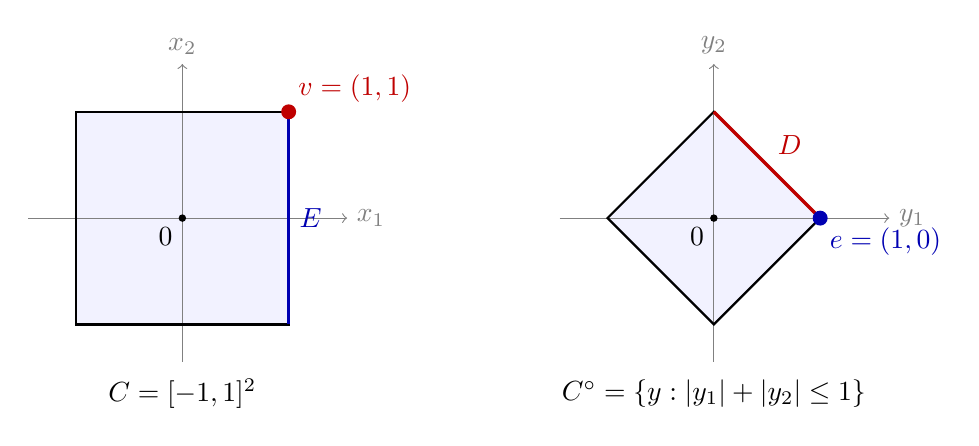
\begin{tikzpicture}[scale=1.35]
	\begin{scope}
		\fill[blue!5] (-1,-1) rectangle (1,1);
		\draw[->,gray] (-1.45,0)--(1.55,0) node[right] {\(x_1\)};
		\draw[->,gray] (0,-1.35)--(0,1.45) node[above] {\(x_2\)};
		\draw[thick] (-1,-1)--(1,-1)--(1,1)--(-1,1)--cycle;
		\draw[very thick,blue!70!black] (1,-1)--(1,1) node[midway,right] {\(E\)};
		\fill[red!75!black] (1,1) circle(2pt) node[above right] {\(v=(1,1)\)};
		\fill (0,0) circle(1pt) node[below left] {\(0\)};
		\node at (0,-1.65) {\(C=[-1,1]^2\)};
	\end{scope}
	\begin{scope}[xshift=5cm]
		\fill[blue!5] (1,0)--(0,1)--(-1,0)--(0,-1)--cycle;
		\draw[->,gray] (-1.45,0)--(1.65,0) node[right] {\(y_1\)};
		\draw[->,gray] (0,-1.35)--(0,1.45) node[above] {\(y_2\)};
		\draw[thick] (1,0)--(0,1)--(-1,0)--(0,-1)--cycle;
		\draw[very thick,red!75!black] (1,0)--(0,1) node[midway,above right] {\(D\)};
		\fill[blue!70!black] (1,0) circle(2pt) node[below right] {\(e=(1,0)\)};
		\fill (0,0) circle(1pt) node[below left] {\(0\)};
		\node at (0,-1.65) {\(C^\circ=\{y:|y_1|+|y_2|\le1\}\)};
	\end{scope}
\end{tikzpicture}

	\caption[正方形与极体的面对应]{正方形与极体的面对应。蓝边 \(E\) 对应蓝顶点 \(e\)；红顶点 \(v\) 对应红边 \(D\)。包含关系 \(v\in E\) 变为 \(e\in D\)。两幅图使用各自的坐标平面。}
	\label{g1:fig:square-polar}
\end{figure}

这种对应不仅存在于平面图形。原点位于内部时，每个支撑值都可以归一化成一，从而把一个面的外法向方向截成极体上的面。

\begin{proposition}[极体的面对应]
	\label{g1:prop:polar-face-duality}
	设 \(P\subseteq\mathbb R^d\) 为满维多胞形，且 \(0\in\operatorname{int}P\)。对非空真面 \(F\)，定义
	\[
		F^*=\{y\in P^\circ:\langle y,x\rangle=1\text{ 对所有 }x\in F\}.
	\]
	它是 \(P^\circ\) 的非空真面，且 \((F^*)^*=F\)。连同约定 \(P^*=\varnothing\)、\(\varnothing^*=P^\circ\)，这给出两个面格之间反转包含关系的双射。对非空真面还有
	\[
		\dim F+\dim F^*=d-1.
	\]
	特别地，顶点对应棱面，棱面对应顶点。
\end{proposition}

\begin{proof}
	选取线性函数 \(\langle u,-\rangle\) 暴露出 \(F\)，即 \(F=F_P(u)\)。因为 \(F\) 为真面，\(u\ne0\)；又因原点在内部，\(h_P(u)>0\)。于是 \(y_0=u/h_P(u)\) 属于 \(P^\circ\)，在 \(F\) 上配对为一，在其他顶点上配对严格小于一。这首先证明 \(F^*\ne\varnothing\)。取 \(F\) 全部顶点的平均点 \(x_0\)。对 \(y\in P^\circ\)，\(\langle y,x_0\rangle=1\) 当且仅当在 \(F\) 的每个顶点都配对为一，也就当且仅当在整个 \(F\) 上配对为一。因此
	\[
		F^*=\{y\in P^\circ:\langle y,x_0\rangle=1\}
	\]
	是一个暴露面。它不含 \(0\)，所以是一个真面。

	由双极公式，\((P^\circ)^\circ=P\)。按定义，\(F\subseteq(F^*)^*\)；若 \(x\in P\setminus F\)，刚才的 \(y_0\) 满足 \(\langle y_0,x\rangle<1\)，又有 \(y_0\in F^*\)，故 \(x\notin(F^*)^*\)。于是 \((F^*)^*=F\)。包含关系的反转直接来自条件“对所有 \(x\in F\)”；再对反向映射应用同一结论，得到反转包含的双射。空面与全体的约定也与包含关系相容。

	最后核对维数。设 \(k=\dim F\)，\(W\) 为 \(F\) 的仿射包络的方向空间，则 \(\dim W=k\)。因 \(F\) 位于支撑超平面 \(\langle y_0,x\rangle=1\) 中，\(x_0\notin W\)。所有对 \(F\) 配对为一的向量组成仿射空间
	\[
		Y=\{y:\langle y,x_0\rangle=1,\ \langle y,w\rangle=0\ (w\in W)\}.
	\]
	这些是 \(k+1\) 个独立线性条件，所以 \(\dim Y=d-k-1\)。在 \(y_0\) 附近、沿 \(Y\) 作足够小的扰动，对 \(F\) 的顶点仍配对为一；对有限个不在 \(F\) 中的顶点，由严格余量，配对仍小于一。因此 \(F^*\) 包含 \(y_0\) 在 \(Y\) 中的一个相对邻域，又完全位于 \(Y\) 内，故 \(\dim F^*=d-k-1\)。
\end{proof}

法锥与极体的面现在也可以直接比较：对非空真面 \(F\) 及 \(x_0\in F\)，有
\[
	F^*=N_P(F)\cap\{y:\langle y,x_0\rangle=1\},\qquad N_P(F)=\{ty:t\ge0,\ y\in F^*\}.
\]
第一个等式把最大值归一化；第二个等式使用了非零外法向量的支撑值严格为正。因而一个面先决定一整束外法向方向，再由极体从每条射线上选取一个代表。原点改变时，归一化的位置也会改变，极体不是单纯由图形的仿射外观决定的。

\subsection{单纯形、立方体和交叉多面体的对照}
\label{g1:subsec:0303:05}

取 \(d\ge2\)。记标准单纯形为 \(\Delta_d=\operatorname{conv}\{0,e_1,\ldots,e_d\}\)，将其重心移到原点后记为 \(S_d\)；另记
\[
	C_d=[-1,1]^d,\qquad O_d=\operatorname{conv}\{\pm e_1,\ldots,\pm e_d\}.
\]
其中 \(\Delta_d\) 是\secref{g1:sec:0101}已经定义的单纯形：它由 \(d+1\) 个仿射无关点生成，维数为 \(d\)。\(C_d\) 是 \(d\) 维立方体，\(O_d\) 称为\term[jiaochaduomianti]{交叉多面体}[cross-polytope]。平移单纯形只是为了满足取有界极体所需的原点条件，不改变其面及包含关系。

\begin{proposition}[三个模型的面数与对偶]
	\label{g1:prop:basic-polytope-counts}
	设 \(d\ge2\)，并以 \(f_k(P)\) 表示 \(P\) 的 \(k\) 维面的数目。则对 \(0\le k\le d-1\)，\cref{g1:tab:basic-polytopes}中的公式成立。其中 \(C_d^\circ=O_d\)、\(O_d^\circ=C_d\)，而 \(S_d^\circ\) 也是一个 \(d\) 维单纯形。
\end{proposition}

\begin{table}[htbp]
	\centering
	\caption[三个基本多胞形的计数与对偶]{三个基本多胞形的计数与对偶。\(0\le k\le d-1\)；每个多胞形另有一个空面和一个全体面。单纯形的极体记为 \(S'_d\)，不表示它与原单纯形逐点相同。}
	\label{g1:tab:basic-polytopes}
	\begin{tabular}{@{}lcccc@{}}
		\toprule
		对象 & 顶点数 & 棱面数 & \(f_k\) & 极体 \\
		\midrule
		单纯形 \(S_d\) & \(d+1\) & \(d+1\) & \(\binom{d+1}{k+1}\) & \(S'_d\) \\
		立方体 \(C_d\) & \(2^d\) & \(2d\) & \(2^{d-k}\binom dk\) & \(O_d\) \\
		交叉多面体 \(O_d\) & \(2d\) & \(2^d\) & \(2^{k+1}\binom d{k+1}\) & \(C_d\) \\
		\bottomrule
	\end{tabular}
\end{table}

\begin{proof}
	单纯形的每个非空面由一部分顶点生成；反过来，任意顶点子集都生成一个面。为说明后一点，使用单纯形上的重心坐标 \(\lambda_0,\ldots,\lambda_d\)：它们是仿射函数，非负且和为一。给定非空真子集 \(I\)，仿射函数 \(\sum_{i\in I}\lambda_i\) 的最大值为一，恰好在其余重心坐标全为零时取得，也就是选定顶点的凸包。仿射函数与其线性部分的最大值集相同，所以这确是一个暴露面。选出 \(k+1\) 个顶点便得到一个 \(k\) 维面，数目为 \(\binom{d+1}{k+1}\)。

	对于立方体，线性函数 \(\sum_i a_ix_i\) 取最大值时，\(a_i>0\) 迫使 \(x_i=1\)，\(a_i<0\) 迫使 \(x_i=-1\)，只有 \(a_i=0\) 的坐标可以自由变化。故 \(k\) 维面由 \(k\) 个自由坐标和其余坐标的 \(\pm1\) 选择确定，共有 \(\binom dk2^{d-k}\) 个。最大值本身是 \(\sum_i|a_i|\)，从而
	\[
		C_d^\circ=\{y:\textstyle\sum_i|y_i|\le1\}=O_d.
	\]
	最后一个等号可以直接核验：\(\sum_i|y_i|\le1\) 时，以 \(|y_i|\) 为系数使用相应符号的 \(e_i\)，剩余权重放在 \(0\)；而 \(0=(e_1+(-e_1))/2\) 本已在这些顶点的凸包中。双极公式给出 \(O_d^\circ=C_d\)。

	对于交叉多面体，非零线性函数 \(\langle a,-\rangle\) 的最大值为 \(M=\max_i|a_i|>0\)，达到最大值的顶点正是 \(\operatorname{sgn}(a_i)e_i\)、\(|a_i|=M\)。它们每个坐标方向至多选一个，且仿射无关。要得到 \(k\) 维面，应选 \(k+1\) 个坐标方向，每个方向任选正负号，共有 \(\binom d{k+1}2^{k+1}\) 种；每种确实能实现，只需让所选坐标的 \(a_i\) 等于相应的 \(\pm1\)，其余为零。

	还需确认平移单纯形的极体也是单纯形，而不只核对面数。置 \(b=(1/(d+1),\ldots,1/(d+1))\)，则 \(S_d=\Delta_d-b\)，故
	\[
		S_d=\{x:-(d+1)x_i\le1\ (1\le i\le d),\ (d+1)\textstyle\sum_i x_i\le1\}.
	\]
	记 \(q_i=-(d+1)e_i\) 和 \(q_0=(d+1)(1,\ldots,1)\)。这些 \(d+1\) 个点仿射无关，且平均为零：若 \(\sum_{i=1}^d c_i(q_i-q_0)=0\)，逐坐标得到 \(c_j=-\sum_i c_i\)，求和即迫使全部系数为零。因此 \(Q=\operatorname{conv}\{q_0,\ldots,q_d\}\) 是含原点的单纯形；上式恰好说明 \(Q^\circ=S_d\)。对闭凸含原点的 \(Q\) 应用双极公式，便有 \(S_d^\circ=Q\)。
\end{proof}

例如三维立方体有 \(8\) 个顶点、\(12\) 条棱和 \(6\) 个棱面，而三维交叉多面体即正八面体，分别有 \(6,12,8\) 个相应的面。两份数目倒序对应，反映的是 \(\dim F+\dim F^*=2\)，不是偶然的数字对称。在一维，单纯形、立方体和交叉多面体都只是线段；在零维，非空多胞形只有一个点，需要在零维环境中单独理解，不能把表中的棱面公式机械延伸过去。

有限表示、面格与极性还可以继续用于研究多胞形的组合结构。按这些主题延伸阅读，可查阅 \cite[Sections 1.1, 2.1--2.4]{Ziegler1995}。

% !TeX root = ../../Book1.tex
% 纲要标题：### 3.4 凸方法在后续几何中的位置
% 纲要位置：几何学计划纲要.md，第 226 行。
% 正文状态：初稿；尚未正式审核。

% 纲要内容开始
% 
% 把支撑函数、对偶锥和格多面体分别接到第三卷距离比较、第四卷矩映射以及第五卷环面簇；这里不调用后续分类定理。
% 
% ---
% 
% 纲要内容结束

\section{凸方法在后续几何中的位置}
\label{g1:sec:0304}

一个凸集可以由它包含的点来描述，也可以由线性函数在它上面的取值界来描述。\cref{g1:prop:support-function-representation}把这两种描述联系起来：只要 \(C\subseteq\mathbb R^n\) 非空、闭且凸，全部不等式 \(\langle u,x\rangle\le h_C(u)\) 就恰好刻画 \(C\)。这一事实不仅能回答“点是否属于集合”，还可以测量点离集合多远。以下仍使用标准欧氏内积与范数，先把这个测量写成一个精确等式。

\begin{proposition}[距离的支撑函数表示]\label{g1:prop:distance-support-formula}
	设 \(C\subseteq\mathbb R^n\) 是非空闭凸集，\(h_C(u)=\sup_{y\in C}\langle u,y\rangle\)。对每个 \(x\in\mathbb R^n\)，有
	\begin{equation}\label{g1:eq:distance-support-formula}
		d(x,C)=\max_{\lVert u\rVert\le1}\bigl(\langle u,x\rangle-h_C(u)\bigr).
	\end{equation}
	当 \(h_C(u)=+\infty\) 时，括号中的值约定为 \(-\infty\)。若 \(x\notin C\)，令 \(p=P_Cx\) 为最近点，则 \(u=(x-p)/\lVert x-p\rVert\) 取得最大值；若 \(x\in C\)，可取 \(u=0\)。
\end{proposition}
\begin{proof}
	对任意 \(y\in C\) 及 \(\lVert u\rVert\le1\)，Cauchy--Schwarz 不等式给出
	\[
		\langle u,x\rangle-h_C(u)\le\langle u,x-y\rangle\le\lVert x-y\rVert.
	\]
	对 \(y\) 取下确界，便知右边的每个候选值都不超过 \(d(x,C)\)。若 \(x\in C\)，取 \(u=0\) 得到 \(0\)，所以等号成立。

	若 \(x\notin C\)，\cref{g1:thm:convex-projection}保证最近点 \(p\) 存在且唯一，并且对所有 \(y\in C\) 有 \(\langle x-p,y-p\rangle\le0\)。令 \(u=(x-p)/\lVert x-p\rVert\)，这条不等式说明 \(h_C(u)=\langle u,p\rangle\)：右侧是所有取值的上界，且在 \(p\in C\) 处达到。因此
	\[
		\langle u,x\rangle-h_C(u)=\langle u,x-p\rangle=\lVert x-p\rVert=d(x,C).
	\]
	这样还直接找到了最大值的取得方向，不需要先假定支撑函数在整个单位球上有限或连续。
\end{proof}

对满足 \(h_C(u)<+\infty\) 的单位向量 \(u\)，超平面 \(\langle u,y\rangle=h_C(u)\) 给出沿该方向的界，\(\langle u,x\rangle-h_C(u)\) 是点 \(x\) 到这个超平面的有向距离。一般情况下上确界未必在 \(C\) 中达到，因此这个超平面未必接触集合；但上面由最近点选出的方向确实给出在 \(p\) 处接触的支撑超平面。对集合外的点，这个方向测得的距离恰好就是到集合的距离。特别地，\(d(\,\cdot\,,C)\) 是凸函数：把每个有限值方向对应的仿射函数在 \((1-t)x+ty\) 处的值展开，再取上确界，就得到
\[
	d((1-t)x+ty,C)\le(1-t)d(x,C)+t\,d(y,C)\qquad(0\le t\le1).
\]
这里取上确界的方向集合与 \(x,y\) 无关，因此每个方向上的仿射等式都受同一个右侧控制。

\begin{example}[球和半空间的距离]\label{g1:exm:support-distance-models}
	对闭球 \(C=\{y:\lVert y-c\rVert\le r\}\)，其中 \(r\ge0\)，有 \(h_C(u)=\langle u,c\rangle+r\lVert u\rVert\)。将它代入\eqref{g1:eq:distance-support-formula}，先沿 \(x-c\) 的方向取 \(u\)，再在 \(0\le\lVert u\rVert\le1\) 中优化，得到
	\[
		d(x,C)=\max\{0,\lVert x-c\rVert-r\}.
	\]
	若 \(x=c\)，直接取 \(u=0\) 即可。对半空间 \(H=\{y:\langle a,y\rangle\le b\}\)，\(a\ne0\)，沿单位法向 \(a/\lVert a\rVert\) 的超出量则给出
	\[
		d(x,H)=\frac{\max\{0,\langle a,x\rangle-b\}}{\lVert a\rVert}.
	\]
	第二式也可直接验证：当 \(x\notin H\) 时，从 \(x\) 减去 \((\langle a,x\rangle-b)a/\lVert a\rVert^2\)，就到达边界上的最近点。
\end{example}

这些计算说明，距离虽然由对所有点求下确界定义，却可以由比较函数从另一侧控制。比如在 \(x_0\notin C\) 处选取上面得到的单位向量 \(u_0\)，仿射函数
\[
	\ell(x)=\langle u_0,x\rangle-h_C(u_0)
\]
满足 \(\ell(x)\le d(x,C)\)，并在 \(x_0\) 处相等。这是一种从下方接触距离函数的比较。第三卷第7章第3、4节将处理曲空间中的距离与割迹，那里的“支撑函数”还指在一点接触目标函数的局部比较函数，不应直接等同于本章定义在方向空间上的 \(h_C\)。比较时究竟从上方还是下方接触、在哪个邻域光滑，以及曲率对二阶导数的限制，都需要另行说明；这里的欧氏公式提供的是一个可以完全算清的模型。

\ProseParagraphBreak

再看同时满足一组齐次不等式的方向。设 \(V\) 是有限维实向量空间。包含 \(0\) 且对非负线性组合封闭的集合 \(C\subseteq V\) 称为\term[tuzhui]{凸锥}[convex cone]；它的\term[duiouzhui]{对偶锥}[dual cone]定义在对偶空间中：
\[
	C^\vee=\{\,\varphi\in V^*:\varphi(v)\ge0\ \text{对所有 }v\in C\,\}.
\]
本节采用非负号约定。选定内积后可以用向量表示线性函数，但 \(v\) 与 \(\varphi\) 原本属于不同空间：一个是允许的方向，另一个是检测该方向的线性量。由定义，\(C^\vee\) 总是闭凸锥。它不是把极体定义中的常数 \(1\) 原样保留的另一种记号；对锥而言，\(\varphi(tv)\le1\) 对所有 \(t\ge0\) 成立，当且仅当 \(\varphi(v)\le0\)，所以前节的极集满足 \(C^\circ=-C^\vee\)。

\begin{proposition}[闭凸锥的双对偶]\label{g1:prop:dual-cone-bipolar}
	设 \(V\) 是有限维实向量空间，\(C\subseteq V\) 是闭凸锥。在自然识别 \(V^{**}=V\) 下，有 \(C^{\vee\vee}=C\)。若
	\[
		C=\left\{\,\sum_{j=1}^m t_jv_j:t_j\ge0\,\right\},
	\]
	则无论是否预先知道此锥闭，都有
	\[
		C^\vee=\{\,\varphi:\varphi(v_j)\ge0,\ j=1,\ldots,m\,\}.
	\]
\end{proposition}
\begin{proof}
	第一式的包含 \(C\subseteq C^{\vee\vee}\) 直接来自定义。若 \(x\notin C\)，由\cref{g1:thm:point-closed-separation}，存在非零线性函数 \(u\)，使 \(u(x)>\sup_{y\in C}u(y)\)，并且右侧有限。因为 \(0\in C\)，该上确界不小于 \(0\)；又因 \(ty\in C\) 对所有 \(t\ge0\) 成立，若某个 \(u(y)>0\)，上确界就会是 \(+\infty\)。故 \(u(y)\le0\) 对所有 \(y\in C\) 成立，且上确界等于 \(0\)。于是 \(-u\in C^\vee\)，而 \((-u)(x)<0\)，排除了 \(x\in C^{\vee\vee}\) 的可能。

	对第二式，\(\varphi\in C^\vee\) 显然在每个生成向量上非负；反之，若这些有限个值都非负，则 \(\varphi(\sum_jt_jv_j)=\sum_jt_j\varphi(v_j)\ge0\)。这正是从全部方向的检验缩减为有限次检验的理由。
\end{proof}

这个定义也解释了为何对偶锥出现在矩映射中。下面的计算只用复数、偏导数和群作用。取整数向量 \(\alpha_1,\ldots,\alpha_N\in\mathbb Z^d\)，记 \(T^d=(\mathbb R/2\pi\mathbb Z)^d\)。在 \(\mathbb C^N\) 上定义作用
\[
	t\cdot(z_1,\ldots,z_N)=
	\bigl(e^{-i\langle\alpha_1,t\rangle}z_1,\ldots,e^{-i\langle\alpha_N,t\rangle}z_N\bigr).
\]
整数条件保证把 \(t\) 的任一坐标加上 \(2\pi\) 不改变作用。定义
\begin{equation}\label{g1:eq:linear-moment-map}
	\mu(z)=\frac12\sum_{j=1}^N|z_j|^2\alpha_j.
\end{equation}
这是此作用的一个\term[juyingshe]{矩映射}[moment map]。要理解名称背后的要求，可把 \(z_j=x_j+iy_j\) 写成实坐标。在两个实切向量 \((a,b)\)、\((c,e)\) 上定义交替配对
\[
	\omega_0((a,b),(c,e))=\sum_j(a_je_j-b_jc_j).
\]
它就是第四卷要使用的标准辛形式 \(\sum_j\mathrm{d}x_j\wedge \mathrm{d}y_j\)，当前只需把它看成明确给定的双线性型。对方向 \(\xi\in\mathbb R^d\)，令 \(\beta_j=\langle\alpha_j,\xi\rangle\)。沿一参数作用 \(s\xi\) 求导，得到速度向量
\[
	X_\xi(z)=\bigl((\beta_jy_j,-\beta_jx_j)\bigr)_{j=1}^N.
\]
而函数 \(H_\xi(z)=\langle\mu(z),\xi\rangle=\frac12\sum_j\beta_j(x_j^2+y_j^2)\) 在方向 \(Y=(c,e)\) 上的导数满足
\[
	\mathrm{d}H_\xi(Y)=\sum_j\beta_j(x_jc_j+y_je_j)=\omega_0(X_\xi,Y).
\]
此外，\(\mu\) 在上述作用下不变，因为每个 \(|z_j|\) 不变。这两个条件是环面作用的矩映射条件在本例中的具体形式。负号放在作用的指数中，是为了与本书 \(\iota_X\omega=\mathrm{d}H\) 的约定相容；若保持 \(\omega_0\) 不变而把作用改成正向旋转，相应的 \(\mu\) 就要变号。一般定义与这些线性例子可参看\cite[Section 5.6]{Cannas2006Symplectic}。

\begin{example}[从权重得到锥与多胞形]\label{g1:exm:moment-cone-polytope}
	对\eqref{g1:eq:linear-moment-map}，非负系数 \(|z_j|^2/2\) 可以独立取遍所有非负实数，故
	\[
		\mu(\mathbb C^N)=\operatorname{cone}(\alpha_1,\ldots,\alpha_N).
	\]
	对任意 \(u\in\mathbb R^d\)，函数 \(\langle u,\mu(z)\rangle\) 处处非负，当且仅当 \(\langle u,\alpha_j\rangle\ge0\) 对每个 \(j\) 成立：必要性只需令其余坐标为零。因此对偶锥恰好记录了哪些线性组合的矩映射分量不会取负值。

	若限制在球面 \(S=\{z:\sum_j|z_j|^2=2\}\) 上，系数之和变为 \(1\)，从而
	\[
		\mu(S)=\operatorname{conv}\{\alpha_1,\ldots,\alpha_N\}.
	\]
	反向包含也有显式验证：给定 \(t_j\ge0\)、\(\sum_jt_j=1\)，取 \(z_j=\sqrt{2t_j}\) 即可。这里是在计算同一个映射限制到球面后的像，并未把这个奇数维球面当作辛流形。\cref{g1:thm:caratheodory}还说明，像中的每一点都可由至多 \(d+1\) 个非零坐标实现；它并不要求原来的每个原像都只有这么多个非零坐标。
\end{example}

第四卷第10章第1节将把这套定义推广到流形上的群作用，第12章第2、3节再讨论紧连通情形的凸性和从多面体构造几何对象的问题。线性模型中像的凸性直接来自可独立调节的非负系数；一般流形并没有这样一套全局坐标，因此需要新的整体论证。

\ProseParagraphBreak

把实向量空间中的整数点也保留下来，会出现另一类信息。称 \(\mathbb R^d\) 中由一组实基 \(e_1,\ldots,e_d\) 的整数线性组合构成的集合为\term[ge]{格}[lattice]，记为 \(M\)。以格点为顶点的多胞形称为\term[geduobaoxing]{格多胞形}[lattice polytope]，也称格多面体。选择格基后可写 \(M=\mathbb Z^d\)。保持格的线性坐标变换必须是整数矩阵，且逆矩阵仍为整数矩阵；由行列式乘法可知这等价于行列式为 \(1\) 或 \(-1\)。因此一般实可逆线性变换不再是允许的坐标变换。

对 \(m=(m_1,\ldots,m_d)\in M\)，在 \((\mathbb C^*)^d\) 上定义
\[
	\chi^m(z)=z_1^{m_1}\cdots z_d^{m_d}.
\]
所有坐标非零，所以负指数也有意义。这些函数满足 \(\chi^{m+m'}=\chi^m\chi^{m'}\)，把格的加法转成函数的乘法。若 \(P\) 是格多胞形，有限集合 \(A=P\cap M=\{m_0,\ldots,m_r\}\) 就给出映射
\begin{equation}\label{g1:eq:lattice-monomial-map}
	\Phi_A:(\mathbb C^*)^d\longrightarrow\mathbb P^r(\mathbb C),\qquad
	z\longmapsto[\chi^{m_0}(z):\cdots:\chi^{m_r}(z)].
\end{equation}
格点集有限，是因为有界集合中每个整数坐标只有有限种可能；各单项式均非零，故这确实定义了射影点。把全部格点平移同一个 \(a\in M\)，所有坐标都乘上共同的非零因子 \(\chi^a(z)\)，映射不变。若 \(m_i+m_j=m_k+m_l\)，像上便有齐次方程 \(Z_iZ_j=Z_kZ_l\)。这说明多面体中的整数关系如何转成几何方程。

\begin{example}[正方形给出的射影二次曲面]\label{g1:exm:lattice-square-segre}
	取 \(P=[0,1]^2\subseteq\mathbb R^2\)，按 \((0,0),(1,0),(0,1),(1,1)\) 排列格点，则
	\[
		\Phi_A(z,w)=[1:z:w:zw],\qquad Z_0Z_3=Z_1Z_2.
	\]
	不但像包含在这个二次曲面中，它的闭包还等于整个曲面。为证明这一点，把第二章的乘积坐标写成
	\[
		([s_0:s_1],[t_0:t_1])\longmapsto
		[s_0t_0:s_1t_0:s_0t_1:s_1t_1].
	\]
	由\cref{g1:prop:segre-rank-one}，其像恰为上述方程的非零齐次解：坐标排成的 \(2\times2\) 矩阵行列式为零，故可分解为两个非零向量的乘积。两个因子的全部坐标均非零时，分别除以 \(s_0,t_0\) 就得到 \(\Phi_A(z,w)\)。任意一对因子都可以用坐标全非零的因子逼近，因而曲面上的每一点都是这个像的极限；另一方面，齐次多项式的零点集是闭集，极限仍满足方程。这里的闭包结论已经用通常的复射影拓扑证明，不需要预先掌握代数簇理论。
\end{example}

同样，区间 \([0,2]\) 的三个格点给出 \(z\mapsto[1:z:z^2]\)，补齐端点后得到 \(Z_0Z_2=Z_1^2\)，正是第二章的二次射影参数曲线。区间 \([0,1]\) 与 \([0,2]\) 作为实凸集可以伸缩对应，内部格点数却不同，于是给出的射影坐标数和嵌入次数也不同。这就是第五卷第28章需要同时记录凸性与整数结构的原因：第1节由对偶格与锥构造仿射模型，第3节再把格点与线丛的截面联系起来。当前的单项式计算给出了可以直接观察的起点。



\begin{chaptersummary}
	凸包由有限凸组合生成，相对内部则在集合真正占据的仿射空间内衡量内部。对非空闭凸集，最近点的存在来自有限维紧性，唯一性来自距离平方沿线段的严格凸性；投影不等式进一步给出点与闭凸集的严格分离。边界支撑、开凸集的弱分离以及紧集与闭集之间的正间隔分离各有自己的假设。支撑函数允许取 \(+\infty\)，其全部有限不等式仍能完整恢复一个非空闭凸集。

	\ProseParagraphBreak

	有限维性的组合后果来自同一条仿射依赖式。调整已有权重并让一个系数降到零，得到 Carathéodory 定理；把正负系数分开归一化，得到 Radon 分割；再把分割用于“每次少一个条件”的公共点，得到有限族的 Helly 定理。单纯形说明这些数量界一般不能降低；无限族的相交还需要额外的紧性条件。

	\ProseParagraphBreak

	有界多面体恰是有限点集的凸包。活动约束决定顶点和面，线性函数的最大值记录暴露的边界，法锥记录哪些方向看见同一个面。原点在内部时，极体仍为满维多胞形，取极两次恢复原物，面对应反转包含关系并交换维数。单纯形、立方体与交叉多面体分别展示了重心坐标、独立坐标约束和绝对值约束所产生的结构。距离、矩映射和格点构造随后使用的，正是这些不等式、非负组合与对偶关系。
\end{chaptersummary}

\BookExercises
以下各题均附完整解答。分离题先核对闭性、凸性与紧性条件；多面体题同时保留几何维数和所在空间的维数，计算极体前先确认原点的位置。


\begin{exercise}\label{g1:ex:relative-triangle}
	在 \(\mathbb R^3\) 中令 \(p_0=(1,0,0)\)、\(p_1=(0,1,0)\)、\(p_2=(0,0,1)\)，并令 \(C=\operatorname{conv}\{p_0,p_1,p_2\}\)。求 \(\operatorname{aff}C\)、\(\operatorname{int}C\)、\(\operatorname{ri}C\) 与 \(\operatorname{rbd}C\)。再证明：若 \(f:F\rightarrow G\) 为有限维实仿射空间间的仿射同构，\(S\subseteq F\) 非空，则 \(f(\operatorname{ri}S)=\operatorname{ri}(f(S))\)，其中两边的相对内部都在相应仿射包络中计算。
\end{exercise}
\begin{solution}
	三点仿射无关，因为 \(p_1-p_0=(-1,1,0)\)、\(p_2-p_0=(-1,0,1)\) 线性无关。故
	\[
		\operatorname{aff}C=\{(x,y,z):x+y+z=1\},\qquad
		C=\{(x,y,z):x+y+z=1,\ x,y,z\geq0\}.
	\]
	它的普通内部为空，因为三维开球不可能包含于这个平面。若三个坐标都为正，在平面内充分小的邻域中它们仍为正，所以这些点属于相对内部。若某个坐标为零，可在平面内作任意小的扰动使该坐标为负，同时调整另一个坐标保持总和为 \(1\)，因此该点不属于相对内部。于是
	\[
		\operatorname{ri}C=\{(x,y,z):x+y+z=1,\ x,y,z>0\},
	\]
	而相对边界由 \(C\) 中至少一个坐标为零的点组成，即三条闭边的并。

	对于一般仿射同构 \(f\)，它与逆映射都保持仿射组合，故 \(f(\operatorname{aff}S)=\operatorname{aff}(f(S))\)。在有限维坐标中，\(f\) 及其逆映射都是线性映射加平移，因而连续；因此这一限制是两个仿射包络之间的同胚。若 \(x\in\operatorname{ri}S\)，它在 \(\operatorname{aff}S\) 中有一个包含于 \(S\) 的开邻域，其像便是 \(f(x)\) 在像仿射包络中包含于 \(f(S)\) 的开邻域。反过来对 \(f^{-1}\) 使用同一论证，得到相等。这个结论只用到仿射同构，未要求 \(S\) 凸。
\end{solution}

\begin{exercise}\label{g1:ex:halfspace-projection}
	设 \(a\in\mathbb R^n\setminus\{0\}\)、\(b\in\mathbb R\)，令 \(H=\{y:\langle a,y\rangle\leq b\}\)。证明
	\[
		P_Hx=x-\frac{\max\{\langle a,x\rangle-b,0\}}{\lVert a\rVert^2}a.
	\]
	再求到闭正象限 \(Q=\{y:y_i\geq0\ (1\leq i\leq n)\}\) 的投影和距离，并说明 \(P_Q\) 为什么一般不是线性映射。
\end{exercise}
\begin{solution}
	若 \(\langle a,x\rangle\leq b\)，则 \(x\in H\)，最近点就是 \(x\)，公式成立。若 \(\langle a,x\rangle>b\)，置 \(t=(\langle a,x\rangle-b)/\lVert a\rVert^2>0\)、\(p=x-ta\)。有 \(\langle a,p\rangle=b\)，故 \(p\in H\)。任取 \(y\in H\)，
	\[
		\langle x-p,y-p\rangle=t(\langle a,y\rangle-b)\leq0.
	\]
	由\cref{g1:thm:convex-projection}，\(p=P_Hx\)。这项计算也给出 \(d(x,H)=\max\{\langle a,x\rangle-b,0\}/\lVert a\rVert\)。

	对正象限，距离平方为 \(\sum_i(x_i-y_i)^2\)，每个坐标的约束互相独立。若 \(x_i\geq0\)，取 \(y_i=x_i\) 使该项为零；若 \(x_i<0\)，对 \(y_i\geq0\) 有 \((x_i-y_i)^2\geq x_i^2\)，且仅在 \(y_i=0\) 时取等号。因此
	\[
		(P_Qx)_i=\max\{x_i,0\},\qquad
		d(x,Q)=\left(\sum_{i:x_i<0}x_i^2\right)^{1/2}.
	\]
	例如 \(P_Q(e_1)=e_1\) 而 \(P_Q(-e_1)=0\)，不满足线性映射必须具有的 \(P_Q(-e_1)=-P_Q(e_1)\)。
\end{solution}

\begin{exercise}\label{g1:ex:nonexpansive-projection}
	设 \(C\subseteq\mathbb R^n\) 非空、闭且凸。证明对所有 \(x,y\in\mathbb R^n\)，
	\[
		\lVert P_Cx-P_Cy\rVert^2\leq\langle P_Cx-P_Cy,x-y\rangle,
		\qquad\lVert P_Cx-P_Cy\rVert\leq\lVert x-y\rVert.
	\]
	再证明，对任意非空集合 \(S\subseteq\mathbb R^n\)，距离函数都满足 \(\lvert d(x,S)-d(y,S)\rvert\leq\lVert x-y\rVert\)；这一步不要求 \(S\) 闭或凸。
\end{exercise}
\begin{solution}
	置 \(p=P_Cx\)、\(q=P_Cy\)。对两次投影分别使用式\eqref{g1:eq:convex-projection-variation}，得到 \(\langle x-p,q-p\rangle\leq0\) 与 \(\langle y-q,p-q\rangle\leq0\)。将第一式反号后与第二式比较，有
	\[
		0\leq\langle x-p,p-q\rangle-\langle y-q,p-q\rangle
		=\langle x-y,p-q\rangle-\lVert p-q\rVert^2,
	\]
	即第一项结论。再用内积不等式，\(\lVert p-q\rVert^2\leq\lVert p-q\rVert\cdot\lVert x-y\rVert\)。当 \(p=q\) 时第二项结论直接成立；否则除以正数 \(\lVert p-q\rVert\) 即可。这说明输入点略有移动时，最近点的移动不会更大。

	对于一般非空 \(S\)，任给 \(\varepsilon>0\)，可取 \(s\in S\) 使 \(\lVert y-s\rVert<d(y,S)+\varepsilon\)。三角不等式给出
	\[
		d(x,S)\leq\lVert x-s\rVert\leq\lVert x-y\rVert+\lVert y-s\rVert
		<\lVert x-y\rVert+d(y,S)+\varepsilon.
	\]
	令 \(\varepsilon\to0^+\)，再交换 \(x,y\)，得到绝对值不等式。选择近似最近点而不是要求真正最近点，正是能够去掉闭性假设的原因。
\end{solution}

\begin{exercise}\label{g1:ex:nonclosed-convex-image}
	取\cref{g1:exm:zero-distance-separation}中的闭凸集 \(B=\{(x,y):x>0,\ y\geq1/x\}\)，令 \(\pi:\mathbb R^2\rightarrow\mathbb R\) 为 \(\pi(x,y)=x\)。求 \(\pi(B)\) 及其闭包的支撑函数，并说明这给“线性映射保持闭凸集”与“支撑函数确定所有凸集”各提供了什么反例。
\end{exercise}
\begin{solution}
	每个 \((x,y)\in B\) 都满足 \(x>0\)；反过来，每个 \(x>0\) 都有 \((x,1/x)\in B\)。因此 \(\pi(B)=(0,\infty)\)，是凸集却不是闭集，它的闭包为 \([0,\infty)\)。这说明线性映射虽然保持凸性，但不一定保持闭性，甚至正交投影到坐标轴也不能保证闭性。

	把 \(u\in\mathbb R\) 看作一维方向，直接取上确界得
	\[
		h_{(0,\infty)}(u)=h_{[0,\infty)}(u)
		=\begin{cases}0,&u\leq0,\\+\infty,&u>0.\end{cases}
	\]
	当 \(u<0\) 时，第一个集合只在 \(x\to0^+\) 时趋近上确界，第二个集合则在 \(x=0\) 取得上确界；支撑函数记录的都是同一个数 \(0\)。所以它并不记录某个边界点是否被删除，无法仅凭这项函数区分两个不同的凸集。闭凸集表示定理中的闭性不能省去。
\end{solution}

\begin{exercise}\label{g1:ex:dense-support-directions}
	设 \(C\subseteq\mathbb R^n\) 为非空紧凸集，\(E\) 为单位球面中的稠密子集。证明
	\[
		C=\bigcap_{u\in E}\{x:\langle x,u\rangle\leq h_C(u)\}.
	\]
	证明闭单位圆盘不能只用有限个方向的支撑半平面表示。最后给出一个非空闭凸集和一个单位圆周中的稠密方向集，说明第一个结论在没有紧性时可能失败。
\end{exercise}
\begin{solution}
	由于 \(C\) 紧，可取 \(R\geq0\) 使 \(\lVert c\rVert\leq R\) 对每个 \(c\in C\) 成立。于是
	\[
		\langle c,u\rangle\leq\langle c,v\rangle+R\lVert u-v\rVert
		\leq h_C(v)+R\lVert u-v\rVert.
	\]
	对 \(c\) 取上确界，再交换 \(u,v\)，得 \(\lvert h_C(u)-h_C(v)\rvert\leq R\lVert u-v\rVert\)，故支撑函数连续。若 \(x\) 满足 \(E\) 中所有方向的支撑不等式，对任意单位向量 \(u\) 选择 \(u_j\in E\) 且 \(u_j\to u\)，取极限得到 \(\langle x,u\rangle\leq h_C(u)\)。由正齐次性，不等式对所有非零方向成立，零方向也成立。\cref{g1:prop:support-function-representation}因此给出 \(x\in C\)。反向包含由支撑函数定义成立。

	对平面闭单位圆盘，单位方向 \(u\) 的支撑值为 \(1\)。给定有限个单位方向 \(u_1,\ldots,u_m\)，选择不同于它们的一个单位向量 \(z\)。则 \(\langle z,u_i\rangle<1\) 对所有 \(i\) 成立。因为只有有限个严格不等式，可以取充分接近 \(1\) 的 \(t>1\)，使 \(\langle tz,u_i\rangle\leq1\) 对每个 \(i\) 仍成立；例如令 \(M=\max_i\langle z,u_i\rangle<1\)，若 \(M>0\) 就取 \(1<t<1/M\)，若 \(M\leq0\) 则任意 \(t>1\) 均可。这样 \(tz\) 属于所有给定半平面的交，却在圆盘之外。没有约束的空方向组更不能表示圆盘。

	最后取 \(C=\mathbb R\times\{0\}\)，令 \(E\) 为单位圆周去掉 \((0,1)\) 和 \((0,-1)\) 后的集合。\(E\) 仍稠密，但每个 \(u\in E\) 的第一坐标非零，沿直线 \(C\) 可以使 \(\langle x,u\rangle\) 任意大，所以 \(h_C(u)=+\infty\)。这些方向的半空间没有提供任何约束，其交为整个 \(\mathbb R^2\)。只有被删去的两个法向方向能检测该直线的竖直位置，这说明紧性保证的有限性与连续性在第一个论证中确有作用。
\end{solution}

\begin{exercise}\label{g1:ex:convex-two-moments}
	给定实数 \(t_1,\ldots,t_m\) 与非负权重 \(a_1,\ldots,a_m\)，其中 \(\sum_i a_i=1\)。证明可以只保留至多三个原来的数，并重新选择非负且和为 \(1\) 的权重，使 \(\sum_i a_i t_i\) 与 \(\sum_i a_i t_i^2\) 同时不变。对原数 \(0,1,2,3\) 各取权重 \(1/4\)，给出三点表示，并证明不能只使用两个原数。
\end{exercise}
\begin{solution}
	把 \(t_i\) 提升为平面点 \(q_i=(t_i,t_i^2)\)。所要保留的两个数恰好是 \(\sum_i a_i q_i\) 的两个坐标。由\cref{g1:thm:caratheodory}，这个凸组合可由至多三个 \(q_i\) 表示；投影到两个坐标，便同时保留两个指定的量。

	给定数据的两个量为 \(3/2\) 与 \(7/2\)。在 \(0,1,3\) 上依次取权重 \(1/6,1/2,1/3\)，有
	\[
		0\cdot\frac16+1\cdot\frac12+3\cdot\frac13=\frac32,\qquad
		0^2\cdot\frac16+1^2\cdot\frac12+3^2\cdot\frac13=\frac72.
	\]
	若只用两个不同的原数 \(u<v\)，并要求加权平均为 \(\mu=3/2\)，则两个权重唯一确定为 \((v-\mu)/(v-u)\)、\((\mu-u)/(v-u)\)。它们非负要求 \(u\le3/2\le v\)，故只有四种候选：\((0,2),(0,3),(1,2),(1,3)\)。对应的平方加权平均由恒等式 \(t^2=(u+v)t-uv\)（在 \(t=u,v\) 处成立）分别得到
	\[
		3,\quad \frac92,\quad \frac52,\quad 3.
	\]
	没有一个等于 \(7/2\)。单点表示的平均又只能是某个原数，不可能等于 \(3/2\)，所以三个点确实必需。
\end{solution}

\begin{exercise}\label{g1:ex:radon-explicit}
	令 \(p_1=(0,0),p_2=(3,0),p_3=(2,2),p_4=(0,1)\)。求这四点的全部仿射依赖关系，写出一个 Radon 分割及其公共点，并判断分割是否唯一，交换两组不计。
\end{exercise}
\begin{solution}
	关系 \(\sum_i c_i p_i=0\)、\(\sum_i c_i=0\) 等价于
	\[
		3c_2+2c_3=0,\qquad 2c_3+c_4=0,\qquad c_1+c_2+c_3+c_4=0.
	\]
	以 \(c_3=3s\) 参数化，得到 \((c_1,c_2,c_3,c_4)=s(5,-2,3,-6)\)。取 \(s>0\)，正、负指标给出 \(\{1,3\}\) 与 \(\{2,4\}\)，归一化为
	\[
		\frac58p_1+\frac38p_3=\frac14p_2+\frac34p_4=\left(\frac34,\frac34\right).
	\]
	这就是两条对角线的交点。任何 Radon 分割若给出两凸组合相等，相减便是一个非零仿射依赖关系。这里所有这样的关系都是上述向量的非零倍数，且四个系数都非零；因此两组只能是它的正指标与负指标，分割在交换两组的意义下唯一。
\end{solution}

\begin{exercise}\label{g1:ex:helly-on-line}
	在 \(\mathbb R^n\) 中给定有限个闭球 \(B_i=\{x:\|x-a_i\|\le r_i\}\)，其中 \(r_i\ge0\)，以及直线 \(L=\{p+tv:t\in\mathbb R\}\)，其中 \(\|v\|=1\)。证明：若任意至多两个球与 \(L\) 有共同点，则所有球与 \(L\) 有共同点。写出每个 \(B_i\cap L\) 所对应的参数区间。进一步，在平面中取圆心 \((0,0),(2,0)\)、半径均为 \(\sqrt2\) 的两个闭圆盘，求它们与直线 \(y=1\) 的共同点。
\end{exercise}
\begin{solution}
	记 \(\alpha_i=\langle a_i-p,v\rangle\)，并将 \(a_i-p=\alpha_i v+w_i\)，其中 \(w_i\perp v\)。由正交性，
	\[
		\|p+tv-a_i\|^2=(t-\alpha_i)^2+\|w_i\|^2.
	\]
	若 \(r_i<\|w_i\|\)，交集为空；否则参数构成闭区间
	\[
		I_i=\left[\alpha_i-\sqrt{r_i^2-\|w_i\|^2},\ \alpha_i+\sqrt{r_i^2-\|w_i\|^2}\right].
	\]
	假设保证这些区间非空且两两相交。由\cref{g1:thm:helly}的一维情形，所有 \(I_i\) 有公共参数，对应所有球与 \(L\) 的公共点。也可直接取所有左端点的最大值 \(a\) 和所有右端点的最小值 \(b\)：取得这两个端点的区间相交，故 \(a\le b\)，任取 \(t\in[a,b]\) 即可。

	在给定平面例子中，取 \(p=(0,1),v=(1,0)\)。两圆心到直线的距离都是 \(1\)，区间半长度为 \(\sqrt{2-1}=1\)，故两个参数区间为 \([-1,1]\) 与 \([1,3]\)。唯一公共参数是 \(t=1\)，得到共同点 \((1,1)\)。这里检查两个球就够，是因为未知公共点被限制在一维直线上。
\end{solution}

\begin{exercise}\label{g1:ex:helly-disk-cover}
	设 \(S\) 是平面中的有限非空点集。若 \(S\) 中每个至多含三个点的子集都能被某个半径为 \(1\) 的闭圆盘包含，证明整个 \(S\) 也能被一个这样的圆盘包含。不同子集所用的圆盘允许不同。说明把“三个”改成“两个”后结论不成立。
\end{exercise}
\begin{solution}
	未知量是圆盘中心。对每个 \(p\in S\)，令 \(C_p=\{c\in\mathbb R^2:\|c-p\|\le1\}\)。一个中心 \(c\) 给出的单位闭圆盘包含 \(p\)，当且仅当 \(c\in C_p\)。每个 \(C_p\) 是凸集：若 \(c_1,c_2\in C_p\) 且 \(0\le t\le1\)，由三角不等式，
	\[
		\|(1-t)c_1+tc_2-p\|\le(1-t)\|c_1-p\|+t\|c_2-p\|\le1.
	\]
	题设恰好说任意至多三个 \(C_p\) 有非空交集。由\cref{g1:thm:helly}的二维情形，全部 \(C_p\) 有公共中心，此中心的单位闭圆盘包含整个 \(S\)。

	反例取 \(S=\{(-1,0),(1,0),(0,\sqrt3)\}\)。三条边的长度均为 \(2\)，每对点可被以其中点为中心的单位闭圆盘包含。若一个中心 \((u,v)\) 到前两点的距离都不超过 \(1\)，则
	\[
		(u+1)^2+v^2\le1,\qquad (u-1)^2+v^2\le1.
	\]
	相加得 \(u^2+v^2\le0\)，所以中心只能是 \((0,0)\)，但它到第三点的距离为 \(\sqrt3>1\)。因此三个点不能同处于一个单位闭圆盘中。
\end{solution}

\begin{exercise}
	\label{g1:exr:clipped-square}
	设 \(P=[-1,1]^2\cap\{(x_1,x_2):x_1+x_2\le1\}\)。求其顶点与棱面，求顶点 \((1,0)\) 的外法锥，并给出 \(P^\circ\) 的顶点表示。
\end{exercise}

\begin{solution}
	原正方形的右上角被直线 \(x_1+x_2=1\) 截去。新直线分别与右边、上边交于 \((1,0)\)、\((0,1)\)，所以候选顶点为
	\[
		(-1,-1),\quad (1,-1),\quad (1,0),\quad (0,1),\quad (-1,1).
	\]
	在每个列出的点都有两条法向量线性无关的限制取等号，故由\cref{g1:thm:polytope-hv}证明中的顶点判别，它们确是顶点。任何其他点至多有一条独立限制取等号，不能成为顶点。五个棱面就是上述相邻顶点连接而成的五条边，其所在直线依次为 \(x_2=-1\)、\(x_1=1\)、\(x_1+x_2=1\)、\(x_2=1\)、\(x_1=-1\)。

	记 \(v=(1,0)\)。若 \(u=(a,b)\in N_P(v)\)，把相邻顶点 \((1,-1)\) 和 \((0,1)\) 代入法锥定义，得到
	\[
		-b\le0,\qquad -a+b\le0,
	\]
	也就是 \(a\ge b\ge0\)。反过来，此时对任意 \(x\in P\)，有
	\[
		\langle u,x-v\rangle=(a-b)(x_1-1)+b(x_1+x_2-1)\le0.
	\]
	所以
	\[
		N_P(v)=\{(a,b):a\ge b\ge0\}=\{s(1,0)+t(1,1):s,t\ge0\}.
	\]
	这说明这个角的外法锥由两条相邻边的外法向生成。

	令 \(Q=\operatorname{conv}\{e_1,-e_1,e_2,-e_2,(1,1)\}\)。由极集的定义，\(Q^\circ\) 的不等式恰好是 \(P\) 的五条限制，所以 \(Q^\circ=P\)。\(Q\) 是闭凸且含原点的集合，双极公式给出
	\[
		P^\circ=Q=\operatorname{conv}\{(1,0),(-1,0),(0,1),(0,-1),(1,1)\}.
	\]
	这些点全都是顶点：\((1,1)\) 唯一最大化 \(y_1+y_2\)，\((1,0)\) 唯一最大化 \(2y_1-y_2\)，\((0,1)\) 唯一最大化 \(-y_1+2y_2\)，而 \((-1,0)\)、\((0,-1)\) 分别唯一最大化 \(-y_1\)、\(-y_2\)。
\end{solution}

\begin{exercise}
	\label{g1:exr:segment-ambient-polar}
	设 \(S=[-1,1]\times\{0\}\subseteq\mathbb R^2\)。写出其半空间表示和全部面，求 \(N_S(S)\)、\(N_S(\{(1,0)\})\) 及环境极集 \(S^\circ\)。再在直线 \(L=\mathbb R\times\{0\}\) 中重复这些计算，说明差异来自哪里。
\end{exercise}

\begin{solution}
	半空间表示为
	\[
		-1\le x_1\le1,\qquad x_2\le0,\qquad -x_2\le0.
	\]
	全部面是 \(\varnothing\)、两个端点单点集以及 \(S\) 本身。事实上，若一个面含有线段的某个内点，面的性质迫使两个端点都在其中，凸性再迫使它等于 \(S\)。

	若线性函数 \(ax_1+bx_2\) 在全部 \(S\) 上达到最大值，它沿 \(x_1\) 方向必须恒定，故 \(a=0\)，而 \(b\) 任意。因此
	\[
		N_S(S)=\{(0,b):b\in\mathbb R\}.
	\]
	若只要求在 \((1,0)\) 取最大值，则条件为 \(a(x_1-1)\le0\) 对 \(-1\le x_1\le1\) 成立，等价于 \(a\ge0\)。所以
	\[
		N_S(\{(1,0)\})=\{(a,b):a\ge0,\ b\in\mathbb R\}.
	\]
	极集要求 \(\sup_{|x_1|\le1}ax_1=|a|\le1\)，故
	\[
		S^\circ=\{(a,b):|a|\le1,\ b\in\mathbb R\},
	\]
	是无界条带。在 \(L\) 中只允许法向量也属于 \(L\)，上述三个集合分别变为 \(\{0\}\)、非负半轴和 \([-1,1]\times\{0\}\)。面本身没有改变；消失的是所有垂直于 \(L\) 的方向。它们在 \(S\) 上的配对恒为零，环境极集无法用不等式约束这些分量。
\end{solution}

\begin{exercise}
	\label{g1:exr:polar-transformation}
	设 \(K\subseteq\mathbb R^n\) 为非空紧凸集，\(T\) 为可逆线性变换，\(a\in\mathbb R^n\)。证明
	\[
		(TK)^\circ=T^{-\mathsf T}K^\circ,\qquad (K+a)^\circ=\{y:h_K(y)+\langle y,a\rangle\le1\}.
	\]
	计算矩形 \([-2,2]\times[-3,3]\) 的极体；再以区间为例说明平移后的极集通常不是原极集的相同平移。
\end{exercise}

\begin{solution}
	由内积与转置的关系，\(y\in(TK)^\circ\) 当且仅当
	\[
		\langle y,Tx\rangle=\langle T^{\mathsf T}y,x\rangle\le1\qquad(x\in K),
	\]
	即 \(T^{\mathsf T}y\in K^\circ\)。乘以逆变换即得第一式。第二式来自
	\[
		\max_{x\in K}\langle y,x+a\rangle=h_K(y)+\langle y,a\rangle.
	\]
	矩形是正方形经 \(T=\operatorname{diag}(2,3)\) 的像，所以其极体为
	\[
		\{(y_1,y_2):2|y_1|+3|y_2|\le1\},
	\]
	顶点是 \((\pm1/2,0)\)、\((0,\pm1/3)\)。长轴方向在取极以后变短，原因是原集合沿该方向越远，相应线性函数允许的系数就越小。

	取 \(K=[-1,1]\)、\(a=1/2\)。则 \(K+a=[-1/2,3/2]\)，正数 \(y\) 要满足 \((3/2)y\le1\)，负数 \(y\) 要满足 \((-1/2)y\le1\)，从而
	\[
		(K+a)^\circ=[-2,2/3].
	\]
	而 \(K^\circ+a=[-1/2,3/2]\)，二者不同。这也说明，即使平移前后原点都在内部，极体仍然依赖所选原点。
\end{solution}

\begin{exercise}
	\label{g1:exr:polar-intersection-hull}
	设 \(K,L\subseteq\mathbb R^n\) 为紧凸集，且 \(0\) 同时在二者内部。证明
	\[
		\bigl(\operatorname{conv}(K\cup L)\bigr)^\circ=K^\circ\cap L^\circ,\qquad (K\cap L)^\circ=\operatorname{conv}(K^\circ\cup L^\circ).
	\]
	用 \(K=[-2,2]\times[-1,1]\)、\(L=[-1,1]\times[-2,2]\) 核验第二式。
\end{exercise}

\begin{solution}
	一个线性函数在 \(\operatorname{conv}(K\cup L)\) 上不超过一，当且仅当它在 \(K\) 和 \(L\) 上分别不超过一，故第一式直接成立。

	证明第二式时需要确保再次取极不会丢失原集合。由\cref{g1:thm:bipolar}的球夹逼，\(K^\circ,L^\circ\) 仍为紧凸集，并含原点为内点。令 \(Q=\operatorname{conv}(K^\circ\cup L^\circ)\)。因为两个集合各自凸，任意混合凸组合都可按来自哪个集合归组，故
	\[
		Q=\{(1-t)y+tz:0\le t\le1,\ y\in K^\circ,\ z\in L^\circ\}.
	\]
	这是紧集 \([0,1]\times K^\circ\times L^\circ\) 在连续映射下的像，所以 \(Q\) 紧，特别是闭。对第一式应用双极公式，有
	\[
		Q^\circ=(K^\circ)^\circ\cap(L^\circ)^\circ=K\cap L.
	\]
	由于 \(Q\) 闭、凸且含原点，再取一次极便得 \((K\cap L)^\circ=Q\)。

	例中 \(K\cap L=[-1,1]^2\)，其极体是 \(D=\{|y_1|+|y_2|\le1\}\)。另一方面，
	\[
		K^\circ=\{2|y_1|+|y_2|\le1\},\qquad L^\circ=\{|y_1|+2|y_2|\le1\}.
	\]
	二者都在 \(D\) 内；\(K^\circ\) 含 \(\pm e_2\)，\(L^\circ\) 含 \(\pm e_1\)，所以它们的凸包包含 \(D\) 的全部顶点，也就包含 \(D\)。两向包含给出所需等式。
\end{solution}

\begin{exercise}
	\label{g1:exr:cube-face-join}
	在 \(C_3=[-1,1]^3\) 中，令 \(v=(1,1,1)\)、\(w=(-1,1,1)\)。求面格中的 \(\{v\}\vee\{w\}\) 与 \(\{v\}\vee\{-v\}\)，并在极体 \(O_3\) 中计算对应面的交，核对包含关系反转。
\end{exercise}

\begin{solution}
	包含 \(v,w\) 的面必须包含线段 \([v,w]\)。该线段本身是立方体的棱：它是线性函数 \(x_2+x_3\) 的最大值集。因此
	\[
		\{v\}\vee\{w\}=[-1,1]\times\{1\}\times\{1\}.
	\]
	若一个面含有 \(v,-v\)，则由凸性含有原点。对任意 \(z\in C_3\)，还有 \(-z\in C_3\)，而 \(0=(z+(-z))/2\)。面的线段性质迫使 \(z\) 属于该面，所以这个面只能是整个 \(C_3\)。故 \(\{v\}\vee\{-v\}=C_3\)，尽管两个点的凸包只是一条体对角线。

	由极面对偶的定义，
	\[
		\{v\}^*=\operatorname{conv}\{e_1,e_2,e_3\},\qquad \{w\}^*=\operatorname{conv}\{-e_1,e_2,e_3\}.
	\]
	第一个三角形中 \(y_1\ge0\)，第二个中 \(y_1\le0\)，所以交集要求 \(y_1=0\)；余下条件是 \(y_2,y_3\ge0\)、\(y_2+y_3=1\)。因此交集恰为 \(\operatorname{conv}\{e_2,e_3\}\)，也是原棱的极对偶面。另一方面，\(\{-v\}^*=\operatorname{conv}\{-e_1,-e_2,-e_3\}\)。这个三角形上的坐标和为 \(-1\)，而 \(\{v\}^*\) 上为 \(1\)，二者交集为空，正好对应 \(C_3^*=\varnothing\)。
\end{solution}

\begin{exercise}
	\label{g1:exr:nonexposed-point}
	令 \(B=\{(x_1,x_2):x_1^2+x_2^2\le1\}\)、\(p=(2,0)\)，并置 \(K=\operatorname{conv}(B\cup\{p\})\)。证明 \(q=(1/2,\sqrt3/2)\) 是 \(K\) 的极点，但 \(\{q\}\) 不是暴露面。指出多胞形的面定理为何不能应用于这个例子。
\end{exercise}

\begin{solution}
	注意 \(\lVert q\rVert=1\) 且 \(\langle q,p\rangle=1\)。在单位圆盘上，Cauchy--Schwarz 不等式给出 \(\langle q,x\rangle\le1\)，等号仅在 \(x=q\) 时成立。因此对 \(K\)，线性函数 \(\langle q,-\rangle\) 的最大值为一，最大值集恰为线段 \([q,p]\)：把 \(K\) 中的点写成 \((1-t)b+tp\)，\(b\in B\)，若 \(t<1\) 且配对为一，就必须有 \(b=q\)。

	假设 \(q=(1-t)x+ty\)，其中 \(x,y\in K\)、\(0<t<1\)。对两边与 \(q\) 配对，得到两个不超过一的数以正权重平均为一，故 \(x,y\in[q,p]\)。而 \(q\) 是这条线段的端点，所以 \(x=y=q\)。这证明 \(q\) 是极点。

	若 \(\{q\}\) 是暴露面，就存在非零 \(u\) 使 \(q\) 成为 \(\langle u,-\rangle\) 在 \(K\) 上的唯一最大值点，因而也是它在 \(B\) 上的最大值点。单位圆盘上线性函数的唯一最大值点是 \(u/\lVert u\rVert\)，所以 \(u=tq\)、\(t>0\)。但这时
	\[
		\langle u,p\rangle=t\langle q,p\rangle=t=\langle u,q\rangle,
	\]
	与唯一性矛盾。因此 \(\{q\}\) 虽然是一个面，却不是暴露面。

	这里的 \(K\) 并非多胞形。例如单位圆左半边每个点 \(r\) 都满足 \(r_1<0\)，函数 \(\langle r,-\rangle\) 在 \(B\) 上唯一最大化于 \(r\)，而 \(\langle r,p\rangle=2r_1<1\)，故在 \(K\) 上仍唯一最大化于 \(r\)。于是 \(K\) 有无穷多个极点，不能由有限点集生成。有限性假设在面定理中确实不可省略。
\end{solution}

\begin{exercise}\label{g1:ex:orthant-distance}
	令 \(C=\mathbb R_{\ge0}^n\)，并定义 \((x_+)_i=\max\{x_i,0\}\)、\((x_-)_i=\max\{-x_i,0\}\)。求 \(P_Cx\)、\(d(x,C)\) 及 \(h_C(u)\)，并在 \(x\notin C\) 时求\eqref{g1:eq:distance-support-formula}的一个最大化方向。
\end{exercise}
\begin{solution}
	平方距离 \(\sum_i(x_i-y_i)^2\) 在约束 \(y_i\ge0\) 下可以逐坐标最小化。当 \(x_i\ge0\) 时取 \(y_i=x_i\)，否则取 \(y_i=0\)，故 \(P_Cx=x_+\)、\(d(x,C)=\lVert x_-\rVert\)。若某个 \(u_i>0\)，令 \(y_i\to+\infty\) 而其余坐标为零，得到 \(h_C(u)=+\infty\)；若所有 \(u_i\le0\)，则 \(\langle u,y\rangle\le0\)，且在 \(y=0\) 处达到零，所以 \(h_C(u)=0\)。当 \(x_-\ne0\) 时，取 \(u=-x_-/\lVert x_-\rVert\)。它是单位向量且各坐标非正，于是
	\[
		\langle u,x\rangle-h_C(u)=\frac{\langle-x_-,x_+-x_-\rangle}{\lVert x_-\rVert}
		=\lVert x_-\rVert.
	\]
	这里 \(\langle x_-,x_+\rangle=0\)，因为每一坐标不可能同时有非零的正部与负部。
\end{solution}

\begin{exercise}\label{g1:ex:cone-lattice-generators}
	在 \(\mathbb R^2\) 中令 \(C=\operatorname{cone}\{(1,0),(1,2)\}\)。
	\begin{enumerate}
		\item 写出 \(C\) 与 \(C^\vee\) 的半空间表示，并给出 \(C^\vee\) 的两个生成向量。
		\item 证明 \(C\cap\mathbb Z^2\) 中每一点都是 \((1,0),(1,1),(1,2)\) 的非负整数线性组合；说明只用原来的两个生成向量为何不够。
	\end{enumerate}
\end{exercise}
\begin{solution}
	1. 写 \((x,y)=s(1,0)+t(1,2)\)，得到 \(y=2t\)、\(x=s+t\)，所以 \(C=\{(x,y):y\ge0,\ 2x-y\ge0\}\)。由生成向量上的有限检验，
	\[
		C^\vee=\{(a,b):a\ge0,\ a+2b\ge0\}.
	\]
	每个这样的 \((a,b)\) 可以写成 \((a/2)(2,-1)+(b+a/2)(0,1)\)，两个系数都非负；反之这两个生成向量均满足不等式。因此 \(C^\vee=\operatorname{cone}\{(2,-1),(0,1)\}\)。

	2. 若 \((x,y)\in C\cap\mathbb Z^2\)，将 \(y\) 除以 \(2\)，写成 \(y=2q+r\)，其中 \(q\ge0\)、\(r\in\{0,1\}\)。由 \(x\ge y/2\) 及 \(x\) 为整数，得 \(x\ge q+r\)，从而
	\[
		(x,y)=(x-q-r)(1,0)+r(1,1)+q(1,2).
	\]
	相反，三个向量的非负整数线性组合显然都属于 \(C\cap\mathbb Z^2\)。原来的两个向量只能产生第二坐标为偶数的整数线性组合，不能产生 \((1,1)\)。因此描述同一个实锥所需的向量，与描述其全部格点加法所需的向量，可以不同。
\end{solution}

\begin{exercise}\label{g1:ex:moment-square-fiber}
	在\eqref{g1:eq:linear-moment-map}中取四个权重 \((0,0),(1,0),(0,1),(1,1)\)，并限制在 \(\sum_{j=0}^3|z_j|^2=2\) 上。证明像为 \([0,1]^2\)，且对给定的 \((a,b)\in[0,1]^2\)，所有可能的四个数 \(t_j=|z_j|^2/2\) 恰为
	\[
		(t_0,t_1,t_2,t_3)=(1-a-b+s,\ a-s,\ b-s,\ s),
	\]
	其中 \(\max\{0,a+b-1\}\le s\le\min\{a,b\}\)。解释为何“凸组合的系数”通常不能唯一确定原像。
\end{exercise}
\begin{solution}
	约束为 \(t_j\ge0\)、\(\sum_jt_j=1\)，而映射值为 \((t_1+t_3,t_2+t_3)\)。令 \(s=t_3\)，解这三个线性等式就得到题中的四元组；非负条件恰好给出所列区间。当 \(0\le a,b\le1\) 时，\(0\le\min\{a,b\}\)，且 \(a+b-1\le a,b\)，所以区间非空。对任意其中的 \(s\)，取 \(z_j=\sqrt{2t_j}\) 就得到所需原像。反过来，任何原像都产生这样的系数，且 \(a=t_1+t_3\)、\(b=t_2+t_3\) 均属于 \([0,1]\)，故像恰为正方形。

	在内部点，例如 \(a=b=1/2\) 处，参数 \(s\) 可以在 \([0,1/2]\) 中变化，已给出不同的模长分配。即使四个 \(t_j\) 都固定，每个非零 \(z_j\) 的复相位仍可改变。因此系数只记录原像的一部分信息，不能把像中的凸组合表示当作原像的唯一坐标。
\end{solution}
